\chapter{Implementación} \label{ich:implementacion}

Las nuevas técnicas que introducimos implican un esfuerzo considerable en la implementación de módulos de código. Como comentamos en \customref{isubsubs:observaciones_conclusiones_pksampling}, el uso de \textit{P-K sampling} provoca que no podamos usar librerías de aprendizaje automático para realizar tareas comunes, como muestreo de datos, funciones de pérdida, métricas, \ldots

Por tanto, en esta sección explicaremos todo el trabajo de implementación realizado.

\section{Control de versiones y buenas prácticas} \label{isec:github_buenas_practicas}

Para el control de versiones, usamos \textit{Git} con \textit{Github}. Todo el desarrollo del trabajo, tanto la implementación de código como la escritura de la presente memoria, se ha realizado en un repositorio abierto alojado en \cite{informatica:repogithub}.

Gracias al uso de \textit{Github} hemos podido implementar fácilmente una serie de buenas prácticas de desarrollo, entre las cuales se encuentran:

\begin{itemize}
    \item El uso de \textbf{\textit{issues}} para especificar las necesidades del proyecto en cada momento, los errores encontrados durante el proceso de implementación, \ldots. Véase por ejemplo \cite{informatica:ejemplo_issue_14}, donde especificamos una necesidad y proponemos una solución. Además, se pueden ver todos los \textit{commits} que tratan con dicha \textit{issue}
    \item Gracias a estar usando \textit{issues}, trabajamos con la metodología de \textbf{\textit{feature branches}}. En esta metodología, por cada nueva característica a implementar, se crea una \textit{branch} de \textit{Git} para introducir los cambios. Una vez se implementa y valida dicha característica, el código de la nueva \textit{branch} se fusiona en la rama principal \cite{informatica:feature_branches}. Como se puede ver en \cite{informatica:repogithub}, el nombre de cada \textit{feature branch} referencia al identificador de la \textit{issue} con la que estamos trabajando
    \item El fusionado de \textit{feature branches} a la rama principal se realiza por medio de \textbf{\textit{pull requests}}. En cada \textit{pull request} podemos revisar el código una última vez antes de fusionarlo en la rama principal. Además, sirven como forma de localizar los cambios de alto nivel introducidos en nuestra base de código. En nuestro caso, los \textit{commits} individuales pueden llegar a ser demasiado granulares, y revisando la lista de todos los \textit{commits} realizados podemos perder el foco sobre la tarea de alto nivel que tratan de resolver. Por ejemplo, en una \textit{pull request} como \cite{informatica:ejemplo_pr_57} podemos ver que, para introducir las dos variantes de \textit{Rank@K accuracy} (véase \customref{isubs:rank_at_k}) empleamos 53 \textit{commits}.
    \item El uso de \textbf{\textit{Github Actions}} para ejecutar ciertas tareas tras realizar una subida de \textit{commits} al repositorio (\entrecomillado{push}) o antes de aceptar una \textit{pull request}. Principalmente, hemos usado estas \entrecomillado{actions} para lanzar todos los \textit{tests} unitarios tras cada \textit{push} al repositorio y lanzar todos los \textit{tests} de integración antes de cada \textit{pull request}. El objetivo de esta base de \textit{tests} se especifica en \customref{isec:test_suite}
    \item El uso de \textbf{\textit{Github Projects}}, que nos ofrecen una tabla tipo \entrecomillado{Kanban} para organizar las tareas pendientes. Dicha forma de organizarnos ha sido ya comentada en \customref{isec:planificacion}.
\end{itemize}

\section{Estructura de carpetas del proyecto} \label{isec:estructura_carpetas}

Por la extensión de la base de código, es necesario que comentemos la estructura de carpetas del proyecto. En el directorio raíz tenemos los siguientes ficheros relevantes:

\begin{itemize}
    \item \lstinline{flake.nix} y \lstinline{flake.lock} especifican el entorno de desarrollo usando el gestor \textit{nix}. El fichero \lstinline{enviroment.yml} especifica el entorno de desarrollo usando el gestor \textit{Conda} (véase \customref{isec:entorno_ejecucion})
    \item Los ficheros \lstinline{interactive_slurm.sh} y \lstinline{launch_server_process.sh} son dos \textit{scripts Bash} que usamos para lanzar procesos en los servidores \textit{nGPU}. El primero lo utilizamos para entrar en una terminal de forma interactiva. El segundo, para lanzar un \textit{script} de \lstinline{Python} para que ejecute el aprendizaje y validación de un modelo
    \item \lstinline{justfile} especifica tareas para ejecutarse con la herramienta \lstinline{just} \cite{informatica:just}. Dicha herramienta es parecida a \lstinline{make}. La usamos para definir tareas como:
        \begin{itemize}
            \item Sincronizar las bases de código entre los tres entornos distintos con los que hemos trabajado
            \item Ejecutar ciertos \textit{scripts}
            \item Ejecutar la \textit{suite} de pruebas y los \textit{benchmarks}
            \item Ejecutar ciertos análisis estáticos sobre la base de código (usando \lstinline{mypy} y \lstinline{ruff})
            \item \ldots
        \end{itemize}
    \item \lstinline{optuna_queries.sql} define las consultas \lstinline{SQL} necesarias para vigilar el proceso de \textit{hyperparameter tuning}, que especificaremos en \customref{isec:hp_tuning}
\end{itemize}

En el directorio raíz del proyecto tenenos los siguientes subdirectorios:

\begin{itemize}
    \item \lstinline{.github/workflows} en el que definimos las \textit{Github Actions} que ejecutamos (véase \customref{isec:github_buenas_practicas})
    \item \lstinline{thesis} donde desarrollamos el proyecto \textit{Latex} que compone la presente memoria
    \item \lstinline{src} donde realizamos todo el desarrollo de código. Este a su vez se divide en los siguientes subdirectorios:
        \begin{itemize}
            \item \lstinline{lib} donde implementamos toda la librería que usamos en los \textit{Notebooks} y en los \textit{scripts} de entrenamiento. Implementan tareas varias, como el cálculo de funciones de pérdida, el \textit{P-K sampling}, métricas, bucles de entrenamiento, el sistema de \textit{logging}, \ldots
            \item \lstinline{test} e \lstinline{integration_tests} donde alojamos toda la \textit{suite} de pruebas unitarias y de integración, para validar las implementaciones realizadas en nuestra librería
            \item \lstinline{benchmarks} donde alojamos los \textit{benchmarks} empleados en \customref{isec:optimizacion_codigo}
            \item \lstinline{profiling} contiene los datos generados en los \textit{benchmarks} y la documentación del proceso de optimización basado en datos
        \end{itemize}
    \item En \lstinline{src} tenemos algunos ficheros relevantes:

        \begin{itemize}
            \item \textit{Jupyter Notebooks} donde realizamos análisis exploratorios de distintas bases de datos
            \item \textit{Scripts} de \lstinline{Python}, usados principalmente para entrenar y validar modelos
        \end{itemize}\end{itemize}

\section{Estructura lógica de la base de código} \label{isec:estructura_paquetes_modulos}

En \customref{isec:estructura_carpetas} ya hemos hablado de la estructura de carpetas de la base de código. Ahora pasamos a comentar la estructura lógica de la base de código. Nos centraremos en la parte de la librería, pues en los \textit{Notebooks} y \textit{scripts} de \lstinline{Python} consumimos la librería para realizar análisis exploratorio de datos, entrenamiento de modelos y validación (véase \customref{isec:pipeline}).

Empezamos mostrando el diagrama de paquetes de nuestra librería:

\begin{figure}[H]
    \centering
    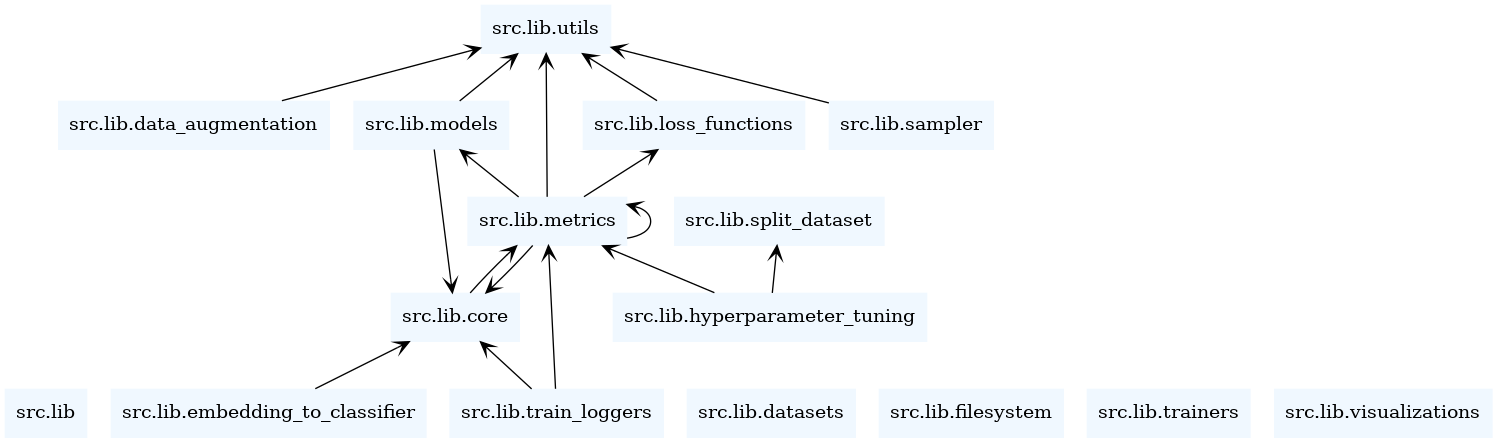
\includegraphics[width=1.0\textwidth]{informatica/diagrama_paquetes}
    \caption{Diagrama de paquetes de nuestra librería. Este diagrama ha sido creado usando la herramienta \lstinline{pyreverse}, que se ofrece como parte del programa \lstinline{pylint}.}
\end{figure}

Como deja claro el diagrama, hemos estructurado el código de la librería en módulos muy interconectados entre ellos. Comentamos ahora el \textbf{propósito de los módulos más relevantes}:

\begin{itemize}
    \item \lstinline{src.lib.utils} contiene funciones auxiliares que se usan en distintas partes del código. Por ejemplo, comprobar si un tensor de \lstinline{pytorch} representa un vector o una matriz, realizar ciertos pre-cómputos para acelerar la ejecución de módulos, autentificarse en el servicio de logging \lstinline{wandb}, \ldots
    \item \lstinline{src.lib.loss_functions} contiene todo el código para computar las distintas funciones de pérdida que hemos introducido en \customref{ich:fundamentos_teoricos}.
    \item \lstinline{src.lib.sampler} contiene el código que implementa el \textit{P-K sampling}
    \item \lstinline{src.lib.metrics} implementa todas las métricas que hemos introducido en \customref{isec:metricas_teoria}
    \item \lstinline{src.lib.train_loggers} contiene la lógica para mostrar las métricas deseadas durante el ciclo de entrenamiento de forma cómoda, modular y extensible
    \item \lstinline{src.lib.datasets} contiene la lógica para descargar, extraer, y cargar en una clase accesible para \lstinline{pytorch} los \textit{datasets} \textit{FG-Net} y \textit{CACD}
    \item \lstinline{src.lib.hyperparameter_tuning} contiene el código necesario para realizar \textit{hyperparameter tuning} usando \textit{K-Fold Cross Validation}, como hemos introducido en \customref{isec:hptuning_kfold_cross_validation}
    \item \lstinline{src.lib.split_dataset} contiene el código para dividir un \textit{dataset} en dos porciones, usando dos técnicas distintas. La primera técnica consiste en separar el \textit{dataset} usando muestreo aleatorio. La segunda técnica consiste en realizar la separación usando muestreo aleatorio, pero asegurando que no existan individuos de una clase en ambos \textit{datasets} simultáneamente
    \item \lstinline{src.lib.data_augmentation} implementa el aumento de datos. Este aumento de datos es necesario porque, como hemos comentado en \customref{isubsubs:observaciones_conclusiones_pksampling}, para realizar \textit{P-K sampling} es necesario que todos los individuos tengan al menos $K$ imágenes asociadas. Realizamos el aumento de datos de forma clásica, añadiendo nuevos elementos a nuestro \textit{dataset}, y de forma \textit{lazy} o perezosa. En el aumento de datos \textit{lazy} no generamos nuevos elementos hasta que estos se solicitan en alguna parte del código. En \customref{isec:aumentado_datos} explicamos esto en detalle
\end{itemize}

Por la gran extensión de la base de código, mostrar el diagrama de clases completo no aporta apenas información. Pero mostraremos los diagramas de clase de ciertos módulos en \customref{isec:modulos_relevantes}, cuando esto aporte información relevante.

\section{Módulos relevantes} \label{isec:modulos_relevantes}

Por la extensión del proyecto no comentaremos cada módulo de código desarrollado. Sin embargo, en esta sección, estudiaremos algunos de los módulos más relevantes.

\subsection{\textit{P-K sampling}}

En \customref{isubs:muestreo_datos_pk_sampling_teoria} hemos introducido nuevas técnicas para computar el \textit{Triplet Loss}. Una parte fundamental de estas técnicas consiste en realizar el \textit{P-K sampling}, que implementamos en el módulo \lstinline{src.lib.sampler}, en la clase \lstinline{CustomSampler}.

\begin{figure}[H]
    \centering
    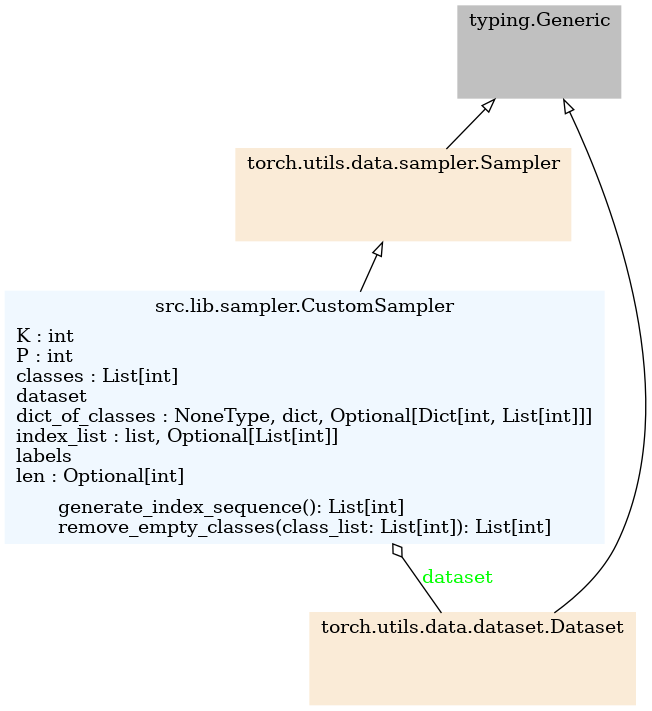
\includegraphics[width=0.6\textwidth]{informatica/pksampler_diagrama_clases}
    \caption{Diagrama de clases de \lstinline{CustomSampler} y sus clases colaboradoras. Este diagrama ha sido creado usando la herramienta \lstinline{pyreverse}, que se ofrece como parte del programa \lstinline{pylint}}
    \label{img:diagrama_clases_CustomSampler}
\end{figure}

En el diagrama de clases \customref{img:diagrama_clases_CustomSampler} podemos ver que:

\begin{itemize}
    \item \lstinline{CustomSampler} hereda de la clase \lstinline{Sampler} de \lstinline{torch} para introducir el comportamiento deseado a través de un \lstinline{Dataloader} \cite{informatica:pytorch_sampler}.
        \begin{itemize}
            \item Un \lstinline{DataLoader} especifica la forma en la que se realiza el \textit{batching} y otros detalles de implementación (por ejemplo, las políticas a seguir para cargar datos cuando trabajamos en paralelo). Uno de sus atributos es el \lstinline{sampler} usado. Escribiendo un \textit{sampler} propio será suficiente para obtener el comportamiento deseado
            \item Un \lstinline{Sampler} indica el orden en el que iteramos un \textit{dataset}. Debe implementar el método \lstinline{__len__()}, que muestra el número de datos que ofrecemos, y el método \lstinline{__iter__()}, que indica cómo se itera sobre los índices de los datos almacenados.
        \end{itemize}
\end{itemize}

En resumen, para realizar \textit{P-K sampling}, especificamos el orden en el que se itera el \textit{dataset} usando la clase \lstinline{CustomSampler}.

Fijados los valores de $P$ y $K$, debemos indicar que el \textit{batch size} sea $P \cdot K$. Esto es claro, pues de otra forma sería imposible generar \textit{batches} en los que haya $P$ individuos representados cada uno con $K$ imágenes.

El funcionamiento de \lstinline{CustomSampler} es el siguiente. Generamos una \textbf{lista de índices} vacía y una lista de imágenes candidatas, que al principio corresponderá al total del \textit{dataset}. Mientras al menos hayan $P$ individuos con al menos $K$ imágenes, realizamos el siguiente proceso:

\begin{enumerate}
    \item Elegimos aleatoriamente $P$ individuos asociados a la lista de imágenes candidatas
    \item Por cada individuo elegido, seleccionamos $K$ imágenes candidatas suyas aleatoriamente
    \item Añadimos los índices asociados a las $P \cdot K$ imágenes escogidas al final de la lista de índices y eliminamos dichas imágenes de la lista de candidatas
\end{enumerate}

Este proceso es realmente sencillo. Sin embargo, realizar optimizaciones para que consuma el menor tiempo posible complica su implementación. Principalmente hemos pre-computado algunos datos, que almacenamos como atributos, para acelerar este proceso:

\begin{itemize}
    \item \lstinline{self.dict_of_classes} es un diccionario en el que cada llave o \textit{key} es el identificador de un individuo (o su clase, en un entorno más amplio que el \textit{AIFR}) y el valor asociado a la llave es una lista de índices de imágenes de ese individuo. Con ello, una vez elegido un individuo al azar, es realmente rápido muestrear $K$ índices de imágenes asociadas
    \item \lstinline{self.classes} es una lista con los identificadores de individuos que tienen al menos $K$ imágenes, y por tanto, que son candidatos a ser elegidos en un ciclo del proceso anteriormente descrito
    \item Esto supone que, durante el proceso de generación de índices, debemos mantener en un estado válido estas dos estructuras, lo que añade algo de complejidad a la implementación, aunque supone una mejora en tiempos de ejecución considerable
\end{itemize}

\begin{observacion}

    Aunque los índices en cada \textit{P-K batch} estén ordenados por individuo, esto no supone un problema al considerar la definición de las funciones de pérdida que estamos usando (véase \customref{isubs:seleccion_de_triples})

\end{observacion}

\subsection{Aumentado de datos} \label{isec:aumentado_datos}

En \customref{isubsubs:observaciones_conclusiones_pksampling} hemos justificado la necesidad de realizar un aumentado de datos en ciertos \textit{datasets}, teniendo mucho cuidado de no saturar la memoria disponible. Por tanto, en el módulo \lstinline{src.lib.data_augmentation} proponemos dos soluciones, que mostramos en el siguiente diagrama de clases:

\begin{figure}[H]
    \centering
    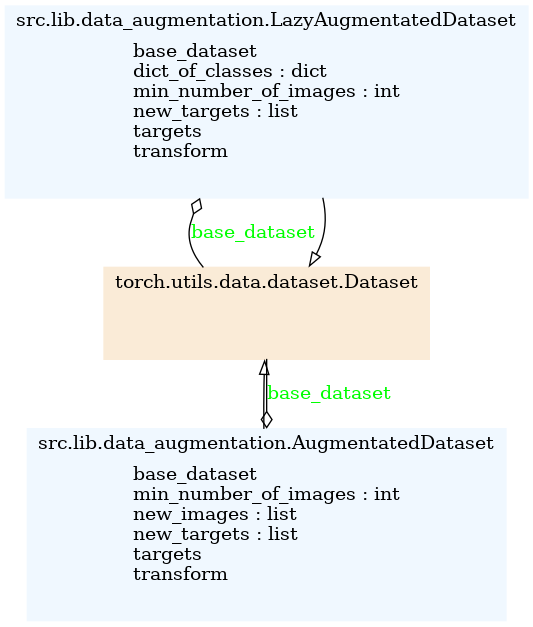
\includegraphics[width=0.6\textwidth]{informatica/diagramas_clases_aumentado_datos}
    \caption{Diagrama de clases de las dos soluciones propuestas para el aumentado de datos. Este diagrama ha sido creado usando la herramienta \lstinline{pyreverse}, que se ofrece como parte del programa \lstinline{pylint}}
    \label{img:diagrama_clases_aumentado_datos}
\end{figure}

En \customref{img:diagrama_clases_aumentado_datos} podemos ver que el aumentado de datos se realiza en dos clases que heredan de la clase \lstinline{Dataset} de \lstinline{pytorch}. Gracias a esto, en nuestros \textit{pipelines} trabajamos igualmente con \textit{datasets} aumentados o sin aumentar, sin conocer este detalle. Además, podemos ver que ambas clases exponen la misma interfaz, por lo que podemos intercambiar estas soluciones. Podemos controlar cómo se generan nuevas imágenes gracias al atributo \lstinline{self.transform}.

Para trabajar con el aumentado de datos, indicamos el \textit{dataset} que queremos aumentar, \lstinline{self.base_dataset}, y el número de imágenes mínimo por individuo, \lstinline{self.min_number_of_images}. Dicho valor siempre lo establecemos igual al valor de $K$ que usemos en cada proceso de entrenamiento. Con ello, aseguramos que cada individuo puede participar en al menos un \textit{P-K batch}.

En \lstinline{AugmentedDataset}, localizamos los individuos con menos de \lstinline{self.min_number_of_images} imágenes asociadas. Generamos y almacenamos en memoria no permanente nuevas imágenes para estos individuos, en base a las imágenes que ya tenemos de los individuos. Almacenamos estas imágenes al final del \textit{dataset} (tienen los índices más altos). Pero esto no supone ningún problema gracias a estar usando \textit{P-K sampling}.

En \lstinline{LazyAugmentedDataset} localizamos los individuos con menos de \lstinline{self.min_number_of_images} imágenes asociadas. Generamos nuevos índices para estos individuos, que almacenamos como atributo, sin computar todavía las nuevas imágenes. Cuando queremos acceder a una imagen concreta identificada por un índice, comprobamos si este índice corresponde a una imagen original o una de las imágenes generadas por el aumento de datos. En el primer caso, devolvemos la imagen que ya tenemos almacenada en el conjunto de datos \lstinline{self.base_dataset}. En el segundo caso, generamos la imagen en ese preciso instante y la devolvemos. En ningún momento almacenamos la nueva imagen para su uso posterior. Por tanto, este aumentado de datos apenas supone un aumento en el uso de memoria \textit{RAM} o memoria \textit{GPU}.

El aumento de datos puede llegar a generar muchísimas imágenes nuevas si la distribución de número de imágenes por individuo es mala (como ocurre en \textit{LFW}, véase \customref{isubsubs:imagenes_por_clase_lfw}). Por tanto, el proceso de almacenar las imágenes que hacemos en \lstinline{AugmentedDataset} puede provocar que saturemos la memoria disponible y que el proceso se detenga. Esto motiva el diseño de \lstinline{LazyAugmentedDataset}, que no almacena imágenes en memoria para su posterior uso.

No almacenar las nuevas imágenes en memoria supone el siguiente compromiso:

\begin{itemize}
    \item Si accedemos dos veces al mismo índice, si este se corresponde con una imagen aumentada, no obtendremos la misma imagen
    \item No se produce un aumento en el consumo de memoria, porque no estamos almacenando ninguna imagen nueva
    \item El proceso de crear un \textit{dataset} aumentado es más rápido. Pero el acceso a nuevos datos es más lento. En la variante \textit{lazy} tenemos que esperar a que se genere la nueva imagen. Mientras que en la variante normal, ese proceso ya se ha realizado previamente y el acceso es inmediato
\end{itemize}

Para realizar el aumento de datos estamos utilizando el módulo \lstinline{torchvision.transforms}. En concreto, usamos las siguientes transformaciones:

\begin{itemize}
    \item Un cortado aleatorio de la imagen, usando \lstinline{RandomResizedCrop}. Dicho método toma una porción aleatoria de la imagen, y cambia su tamaño al especificado en la función. El tamaño de las imágenes producidas es igual al tamaño de las imágenes originales
    \item Una rotación aleatoria, usando \lstinline{RandomRotation}. Rotamos entre 0º y 20º
    \item Un cambio de contraste aleatorio, usando \lstinline{RandomAutocontrast}
\end{itemize}

\subsection{Implementaciones propias de \textit{Datasets}} \label{isec:datasets_customs}

Como ya hemos comentado en \customref{isec:base_datos_usada}, las bases de datos \textit{FG-Net} y \textit{CACD} no se ofrecen como parte de ninguna librería asociada a \lstinline{Pytorch}. Por tanto, tendremos que implementar la descarga, extracción y carga en objetos compatibles con \lstinline{Pytorch}. Estas tareas se realizan en el módulo \lstinline{src.lib.datasets.py}.

Este módulo contiene, además de las dos clases que más adelante estudiamos, las funciones \lstinline{download_fg_dataset} y \lstinline{download_cacd_dataset}, que descargan y extraen los dos \textit{datsets} de internet.

\begin{figure}[H]
    \centering
    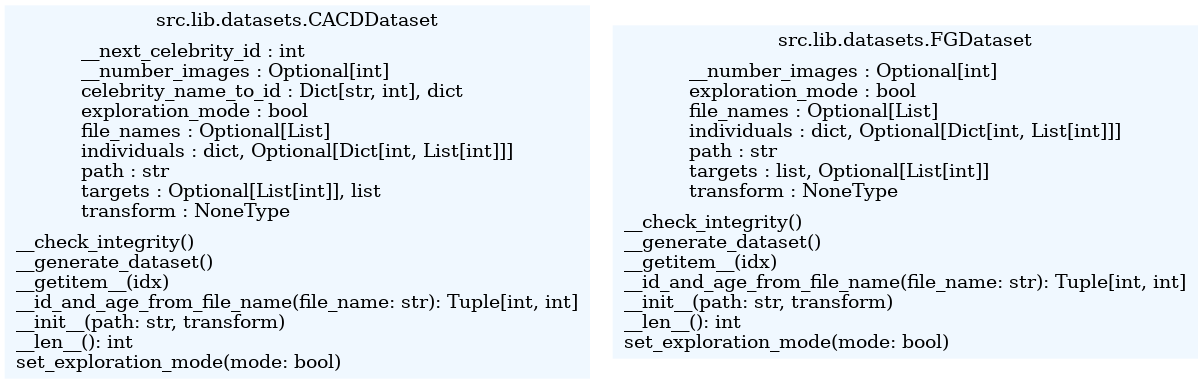
\includegraphics[width=1.0\textwidth]{informatica/diagrama_clases_carga_datos}
    \caption{Diagrama de clases de las implementaciones para los \textit{datasets} \textit{FG-Net} y \textit{CACD}. Este diagrama ha sido creado usando la herramienta \lstinline{pyreverse}, que se ofrece como parte del programa \lstinline{pylint}}
    \label{img:diagrama_clases_datasets}
\end{figure}

En \customref{img:diagrama_clases_datasets} podemos ver el diagrama de clases de las dos implementaciones realizadas. Para inicializar estas clases, solo tenemos que especificar la localización del directorio donde se almacenan los datos.

Para poder trabajar correctamente con \lstinline{Pytorch}, debemos especificar el tamaño del \textit{dataset} con el método \lstinline{__len__()} e implementar el acceso a cada elemento del \textit{dataset} con el método \lstinline{__getitem__()}.

A la hora de cargar los datos al \textit{dataset}, realizamos el siguiente proceso:

\begin{itemize}
    \item Tomamos los nombres de todas las imágenes almacenadas en el \textit{dataset}, que guardamos en el atributo \lstinline{self.file_names}
    \item A partir de los nombres de las imágenes, extraemos el identificador y edad asociados a cada imagen. Para ello usamos el método \lstinline{__id_and_age_from_filename(filename: str)}
    \item Almacenamos adecuadamente toda esta información para poder devolver dicha información en \lstinline{__getitem__}
\end{itemize}

El método \lstinline{check_integrity()} comprueba el tamaño del \textit{dataset} para asegurarnos de que no ha habido corrupción de datos en la descarga. El método \lstinline{set_exploration_mode()} permite activar el modo exploración. En dicho modo, \lstinline{__getitem__()} devuelve la imagen con una serie de metadatos asociados almacenados en un diccionario (edad e identidad). En el modo de funcionamiento normal, \lstinline{__getitem__()} devuelve un par con la imagen y la etiqueta de dicha imagen.

\subsection{Normalización} \label{isubs:normalization_impl}

En \customref{isubs:normalizacion_teoria} hemos justificado por qué es interesante introducir la técnica de normalización en la salida de nuestra red. Además, hemos especificado en qué consiste exactamente esta técnica.

Nuestro objetivo ahora es añadir esta normalización en nuestras redes convolucionales profundas, de forma modular y sencilla. En el módulo \lstinline{src.lib.models}, donde describimos las arquitecturas empleadas a lo largo de toda la experimentación, definimos la clase \lstinline{NormalizedNet}. Dicha clase implementa el patrón de diseño \textit{Decorator} \cite{informatica:design_patterns} \cite{informatica:decorator_pattern}.

En dicho patrón buscamos modificar el comportamiento de un módulo sin cambiar su interfaz. El nuevo comportamiento usa el comportamiento de la clase base, que se adapta de alguna forma. Gracias a no estar modificando la interfaz de la clase base, el resto del código puede trabajar con estos objetos, sin conocer si corresponden a la clase base o a la clase decorada. Esto es justo lo que queremos, porque las funciones que trabajan con nuestra red no deberían depender de la normalización (pensemos por ejemplo en una función que calcula el \textit{Rank@K Accuracy}).

Además, este patrón se basa en la idea de preferir usar composición en vez de herencia (\entrecomillado{composition over inheritance}) \cite{informatica:comp_over_inh}. Mientras que la herencia es estática, la composición es dinámica. Esto, y que el patrón decorador respeta la interfaz de la clase base, permite que podamos combinar varios decoradores a la vez sin problema alguno.

\begin{observacion}

    Este patrón se parece mucho al patrón \textit{Adapter} \cite{informatica:design_patterns} \cite{informatica:adapter_pattern}.

    El objetivo de este patrón es el de adaptar un módulo de código para que implemente una interfaz dada, sin cambiar su comportamiento. Por ejemplo, cuando queremos interactuar con interfaces de terceros usando módulos que no han sido diseñados con dichas interfaces en mente. Por lo tanto, este patrón puede pensarse como el contrario del patrón \textit{Decorator}. Buscamos cambiar la interfaz manteniendo el comportamiento.

\end{observacion}

La clase \lstinline{NormalizedNet} toma una red neuronal como parámetro. Las redes neuronales de \lstinline{pytorch} deben implementar el método \lstinline{forward}, que indica cómo la red computa las salidas a partir de las entradas dadas. Nuestra clase \lstinline{NormalizedNet} implementa este método basándose en el mismo método de la clase base. Usamos el método \lstinline{forward} de la clase base y almacenamos la salida, que normalizamos y devolvemos.

Como ya hemos comentado, el uso de este patrón supone que no estamos cambiando la interfaz de un modelo si lo normalizamos, lo que permite que podamos decidir si queremos trabajar o no con normalización sin que el resto del código tenga que saber este detalle de implementación. Por ejemplo:

\begin{lstlisting}[caption={Ejemplo de uso del patrón \textit{Decorator} para decidir si usamos o no normalización. El resto del código no tiene por qué saber este detalle de implementación, porque no cambiamos la interfaz de la clase}, captionpos=b]
net = LFWResNet18(embedding_dimension = 5)
net = NormalizedNet(net)
\end{lstlisting}

\subsection{\textit{Hyperparameter Tuning}} \label{isec:hp_tuning}

Como hemos comentado en \customref{isec:hptuning_kfold_cross_validation}, usaremos la técnica de \textit{K-Fold Cross Validation} para buscar buenos valores de hiperparámetros. Para facilitar este proceso, desarrollamos un módulo \lstinline{src.lib.hyperparameter_tuning}.

En este módulo definimos la función \lstinline{custom_cross_validation}, cuyo objetivo es implementar la primera componente que mencionamos en \customref{isec:hptuning_kfold_cross_validation}. Por lo tanto, debe generar una métrica a optimizar a partir de una configuración de hiperparámetros dada. La función acepta los siguientes parámetros:

\begin{itemize}
    \item \lstinline{train_dataset}, \textit{dataset} de entrenamiento, sobre el que construiremos los \textit{folds}
    \item \lstinline{k}, número de \textit{folds} a usar. No confundir con el valor de $K$ en \textit{P-K sampling}
    \item \lstinline{random_seed}, valor de la semilla aleatoria, para que los resultados sean reproducibles
    \item \lstinline{network_creator}, función que devuelve una red inicializada aleatoriamente con la arquitectura que queramos trabajar
    \item \lstinline{network_trainer}, función que toma un \textit{dataloader} y una red neuronal, y ejecuta el entrenamiento devolviendo la red entrenada
    \item \lstinline{loader_generator}, función que toma un \textit{dataset} que representa uno de los dos bloques (el \textit{fold} de validación o los $k-1$ \textit{folds} de entrenamiento), el tipo de bloque (entrenamiento o validación) y genera un \lstinline{torch.utils.dada.Dataloader} adecuado para poder lanzar el proceso de entrenamiento y el cálculo de la función a optimizar
    \item \lstinline{loss_function}, función que queremos optimizar usando \textit{hyperparameter tuning}
\end{itemize}

Estamos aplicando el patrón estrategia \cite{informatica:design_patterns} \cite{informatica:strategy_pattern_web}. Pero en vez de estar usando el enfoque clásico en un ambiente de programación orientada a objetos, estamos usando un enfoque funcional. Gracias a esto, podemos usar esta función configurando muy fácilmente qué redes neuronales queremos usar, cómo queremos entrenar la red, cómo queremos trabajar con los datos, ... Y como comentamos a continuación, todo esto de forma dinámica en base a los hiperparámetros propuestos por el \textit{framework} usado (\lstinline{optuna}).

Usando esta función, cada \textit{script} que usemos para entrenar y validar definirá una sección de ajuste de hiperparámetros (como comentamos en \customref{isec:pipeline}). Usaremos el \textit{framework} \lstinline{optuna} para realizar una búsqueda en el espacio de hiperparámetros \cite{informatica:optuna_web}. Este \textit{framework} implementa toda la lógica necesaria para proponer valores de hiperparámetros, y en base a los resultados obtenidos gracias a \lstinline{custom_cross_validation}, proponer nuevos hiperparámetros. Además, usa \lstinline{SQLite} para almacenar los resultados e introducir paralelismo, lo que permite que lancemos varios procesos en los servidores \textit{nGPU}, disminuyendo los tiempos de búsqueda. Como ya hemos comentado, el fichero \lstinline{optuna_queries.sql} contiene las consultas \textit{SQL} para poder acceder a la base de datos donde se almacenan los resultados de la búsqueda.

En la sección de ajuste de hiperparámetros, deberemos configurar \lstinline{optuna} para realizar la búsqueda:

\begin{itemize}
    \item Indicamos qué hiperparámetros queremos explorar, el rango de valores que pueden tomar y sus distribuciones
    \item Configuramos el proceso que produce el valor numérico a optimizar. En nuestro caso, en función de los hiperparámetros elegidos por \lstinline{optuna}, construimos un modelo u otro, adaptamos la red adecuadamente (por ejemplo, añadiendo o no normalización) y lanzamos la función \lstinline{custom_cross_validation} que en definitiva produce la métrica a optimizar
\end{itemize}

En \customref{isec:experimentacion_hp_tuning} usaremos este módulo para realizar la selección de hiperparámetros.

\subsection{Adaptador para realizar \textit{retrieval}} \label{isubs:impl_retr_adapter}

Como hemos comentado en \customref{isec:triplet_loss}, una de las ventajas de que nuestro modelo aprenda un \textit{embedding} semántico es que podemos adaptar dicho modelo para realizar varias tareas. La tarea que nos interesa en este trabajo es la de \textit{retrieval}.

Esta adaptación se realiza en las clases \lstinline{RetrievalAdapter} y \lstinline{FastRetrievalAdapter}, que se encuentran en el módulo \lstinline{src.lib.models}. Mostramos los diagramas de clase asociados:

\begin{figure}[H]
    \centering
    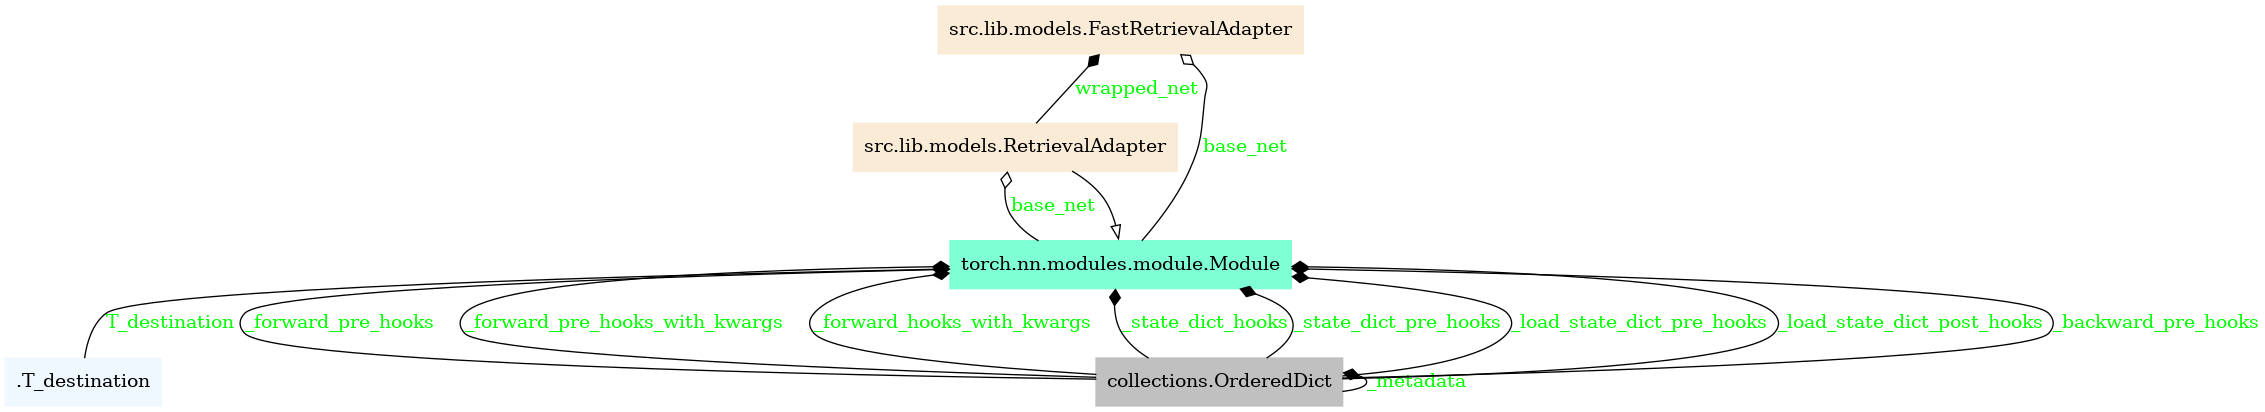
\includegraphics[width=1.0\textwidth]{informatica/diagrama_clases_retrieval}
    \caption{Diagrama de clases de los dos adaptadores. Por el tamaño de \lstinline{torch.nn.Module} solo mostramos los nombres de las clases. Este diagrama ha sido creado usando la herramienta \lstinline{pyreverse}, que se ofrece como parte del programa \lstinline{pylint}}
    \label{img:diagrama_clases_global_adaptadores}
\end{figure}

\begin{figure}[H]
\centering
    \ajustarsubcaptions
    \begin{subfigure}{.6\textwidth}
        \centering
        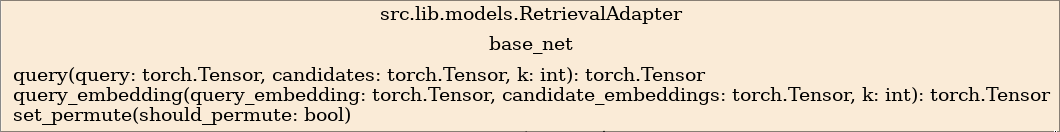
\includegraphics[width=0.9\linewidth]{informatica/diagrama_clases_retrievaladapter}
        \caption{Diagrama de clase de \lstinline{RetrievalAdapter}}
    \end{subfigure}%
    \begin{subfigure}{.4\textwidth}
        \centering
        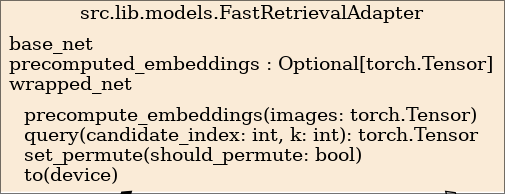
\includegraphics[width=0.9\linewidth]{informatica/diagrama_clases_fastretrieval}
        \caption{Diagrama de clase de \lstinline{FastRetrievalAdapter}}
    \end{subfigure}
\caption{Diagrama de clase de los dos adaptadores, con toda la información asociada. Estos diagramas han sido creados usando la herramienta \lstinline{pyreverse}, que se ofrece como parte del programa \lstinline{pylint}}
\label{img:diagramas_clase_concretos_adaptadores}
\end{figure}

En \customref{img:diagrama_clases_global_adaptadores} podemos ver que ambas clases implementan la interfaz \lstinline{torch.nn.Module}, que es la interfaz que las redes neuronales y sus componentes deben implementar en \lstinline{pytorch}. Además, \lstinline{RetrievalAdapter} forma parte de \lstinline{FastRetrievalAdapter}. Sin embargo, vamos a introducir una nueva interfaz, por lo que queda claro que ahora sí que vamos a usar el patrón \textit{Adapter} (en \customref{isubs:normalization_impl} hablamos de los patrones \textit{Adapter} y \textit{Decorator} en profundidad).

En \customref{img:diagramas_clase_concretos_adaptadores} podemos ver que no estamos buscando trabajar con la interfaz de \lstinline{torch.nn.Module}, sino que buscamos trabajar con una nueva interfaz, asociada a la tarea de \lstinline{retrieval} (véase \customref{ich:descrp_problema}). Para ello, la clase \lstinline{RetrievalAdapter} define dos métodos relevantes, que son los que introducen una nueva interfaz:

\begin{itemize}
    \item \lstinline{query} toma una imagen \textit{key}, una lista de imágenes que forman la base de datos y el número de imágenes $k$ que queremos que devuelva la consulta. Devuelve los índices asociados a las mejores $k$ imágenes de la base de datos
        \begin{itemize}
            \item Tenemos imágenes como entradas, así que debemos almacenar la red neuronal que computa los \textit{embeddings} para transformar estas imágenes
            \item Esto lo hacemos con el atributo \lstinline{self.base_net}
        \end{itemize}
    \item \lstinline{query_embedding} realiza la misma tarea, pero en vez de pasar la imagen \textit{key} y las imágenes que forman la base de datos, pasamos directamente los \textit{embeddings} de estas imágenes. En este caso:
        \begin{itemize}
            \item Tenemos que tener cuidado de usar la misma red neuronal que la que tenemos almacenada en \lstinline{self.base_net}, para evitar errores lógicos
            \item \lstinline{src.base_net} no participa en el cómputo de este método
        \end{itemize}
    \item \lstinline{set_permute} trata sobre detalles sobre como trabajamos la representación de los tensores de \textit{batches} en memoria
\end{itemize}

La clase \lstinline{FastRetrievalAdapter} añade algunas modificaciones para acelerar los tiempos de cómputo:

\begin{itemize}
    \item Podemos ver en \customref{img:diagramas_clase_concretos_adaptadores} que esta clase se compone de un modelo que computa el \textit{embedding} semántico, \lstinline{self.base_net}, y un modelo que ya está adaptado a la tarea de \textit{retrieval}, \lstinline{self.wrapped_net}. \lstinline{self.wrapped_net} es el resultado de construir un objeto de la clase \lstinline{RetrievalAdapter} usando \lstinline{self.base_net}
    \item En \customref{isubs:rank_at_k} se especifica de qué forma se va a usar la adaptación. Siempre tomaremos una base de datos de imágenes, extraeremos una imagen que usaremos como \textit{key}, y realizaremos la \textit{query} contra el resto de imágenes de la base de datos
    \item Por tanto, en el método \lstinline{precompute_embeddings} pasamos toda la base de datos de imágenes, calculamos su proyección en el \textit{embedding} usando \lstinline{self.base_net}, y almacenaremos estos datos
    \item Con esto, el método \lstinline{query} simplemente especifica el índice de la \textit{key} y el número $k$ de individuos más parecidos que queremos seleccionar. Y usando \lstinline{self.wrapped_net} con su método \lstinline{query_embedding}, realizamos el cómputo sobre los \textit{embeddings} precomputados
\end{itemize}

\begin{sloppypar}
\lstinline{FastRetrievalAdapter} claramente está utilizando el patrón \textit{Decorator} (del que ya hemos hablado en \customref{isubs:normalization_impl}) sobre la clase \lstinline{RetrievalAdapter}. Para acelerar los tiempos de ejecución, simplemente realizamos un pre-cómputo y utilizamos la implementación de la clase \lstinline{RetrievalAdapter}.
\end{sloppypar}

\subsection{Separación de datos imponiendo clases disjuntas}

A la hora de separar el \textit{dataset} completo en subconjuntos (entrenamiento, validación y \textit{test}), la opción más utilizada es la de usar muestreo aleatorio para seleccionar qué elementos van a un conjunto u otro. En el problema que estamos resolviendo esto puede no ser adecuado por las siguientes peculiaridades:

\begin{itemize}
    \item Un individuo con al menos $K$ imágenes asociadas puede acabar teniendo menos de $K$ imágenes asociadas en el subconjunto de entrenamiento. Esto provoca que no pueda participar en ningún \textit{P-K batch} en el proceso de aprendizaje
    \item Además, podemos acabar con conjuntos de validación y \textit{test} en los que muchos individuos han sido vistos durante el proceso de entrenamiento. En la aplicación real del modelo vamos a encontrarnos con muchas identidades nunca vistas (potencialmente siempre será así)
\end{itemize}

Por tanto, es conveniente que usemos una separación de datos en la que las identidades (clases, en un ambiente más amplio que el \textit{AIFR}) sean disjuntas. Esto es, que no existan individuos con imágenes asociadas en más de un conjunto de datos.

Las dos técnicas de separación (clásica e identidades disjuntas) se implementan en el módulo \lstinline{src.lib.split_dataset}, en las funciones \lstinline{split_dataset} y \lstinline{split_dataset_disjoint_classes}

\subsection{Logging de métricas} \label{isec:loggin_metricas}

\begin{figure}[H]
    \centering
    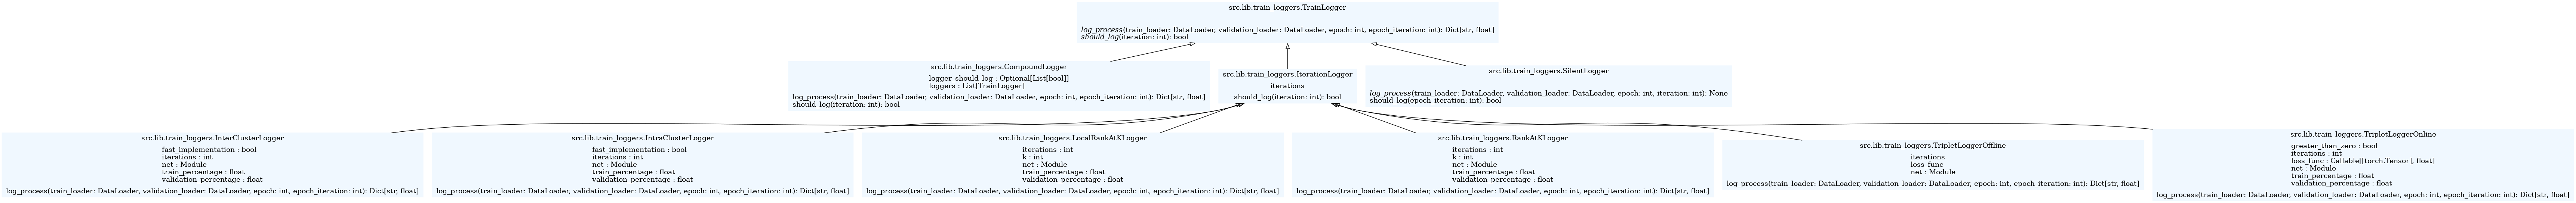
\includegraphics[width=1.0\textwidth,height=\textheight,keepaspectratio]{informatica/diagrama_loggers}
    \caption{Diagrama de clases del módulo \lstinline{src.lib.train_loggers}. Este diagrama ha sido creado usando la herramienta \lstinline{pyreverse}, que se ofrece como parte del programa \lstinline{pylint}}
    \label{img:diagrama_clases_loggers}
\end{figure}

El módulo \lstinline{src.lib.train_loggers} se encarga de introducir el cálculo y visualización de métricas en el proceso de entrenamiento de forma cómoda, modular y extensible. Nuestro objetivo es definir el proceso de \textit{logging} de forma externa al bucle de entrenamiento. Así podremos cambiar las métricas observadas sin tener que modificar el código que implementa el bucle de entrenamiento.

En \customref{img:diagrama_clases_loggers} podemos ver la siguiente estructura:

\begin{itemize}
    \item La clase abstracta \lstinline{Trainlogger} define la interfaz que queremos que todos los \textit{loggers} implementen. Dicha interfaz se compone de dos métodos:
        \begin{itemize}
            \item \lstinline{log_process} que muestra los valores de ciertas métricas tomando como entradas los datos de entrenamiento, los datos de validación, la época en la que nos encontramos en el proceso de entrenamiento y la iteración dentro de dicha épica
            \item \lstinline{should_log} que decide si debemos mostrar o no las métricas para una iteración global del proceso de entrenamiento
        \end{itemize}
    \item Gracias a esta interfaz, el bucle de entrenamiento puede mostrar métricas solo cuando \lstinline{should_log} lo indique, pasando todos los datos necesarios a \lstinline{log_process}
    \item La clase \lstinline{SilentLogger} ofrece una implementación trivial de la interfaz. \lstinline{should_log} siempre devuelve falso y \lstinline{log_process} no realiza ninguna acción
    \item El resto de clases tienen la misma lógica para decidir cuándo mostrar las métricas. Por tanto, la clase abstracta \lstinline{IterationLogger} implementa dicha lógica compartida, dejando todavía como método abstracto a \lstinline{log_process}
    \item Los \textit{loggers} que vemos en la parte baja del diagrama son \textit{loggers} concretos que implementan cada uno \lstinline{log_process} con el cálculo y visualización de métricas concretas
    \item La clase \lstinline{CompoundLogger} implementa el \textbf{patrón de diseño \textit{composite}}
\end{itemize}

Como acabamos de comentar, la clase \lstinline{CompoundLogger} implementa el patrón de diseño \textit{composite} \cite{informatica:design_patterns}. En dicho patrón buscamos definir la lógica de ciertos componentes en función del agregado de otros componentes. En nuestro caso, buscamos definir un objeto que implemente la interfaz \lstinline{TrainLogger} combinando varios \textit{loggers} en uno solo. Para ello, guardamos una lista de objetos de tipo \lstinline{TrainLogger}. La función \lstinline{should_log} consulta a todos los objetos guardados si quieren mostrar métricas, haciendo uso de la misma función \lstinline{should_log}. En cuyo caso, se llama a los correspondientes métodos \lstinline{log_process}. Gracias a esto, en un \textit{script} de \lstinline{Python} podemos configurar nuestro \textit{logging} con el siguiente código:

\begin{lstlisting}[language=python, caption=Ejemplo de configuración del \textit{logging} de un entrenamiento con nuestro sistema propio. Se ve claramente la ventaja de usar un patrón \textit{composite} a la hora de configurar qué \textit{loggers} queremos usar, captionpos=b]

# Define the loggers we want to use
triplet_loss_logger = TripletLoggerOnline(... params ... )
cluster_sizes_logger = IntraClusterLogger(... params ... )
intercluster_metrics_logger = InterClusterLogger( ... params ... )
rank_at_one_logger = RankAtKLogger( ... params ... )
rank_at_k_logger = RankAtKLogger( ... params ... )
local_rank_at_one_logger = LocalRankAtKLogger( ... params ... )
local_rank_at_k_logger = LocalRankAtKLogger( ... params ... )

# Combine them in a single logger
logger = CompoundLogger([
    triplet_loss_logger,
    cluster_sizes_logger,
    intercluster_metrics_logger,
    rank_at_one_logger,
    rank_at_k_logger,
    local_rank_at_one_logger,
    local_rank_at_k_logger,
])
\end{lstlisting}

Hemos usado \textbf{dos técnicas para mostrar las métricas calculadas}. La primera y más sencilla ha sido \textbf{imprimir por pantalla} los valores obtenidos. Esta técnica no es suficiente porque no podemos guardar de forma estructurada los históricos de entrenamientos, ni facilita estudiar de forma visual el comportamiento del entrenamiento. Por tanto, hemos usado como segunda técnica el servicio \textbf{\textit{Weights and Biases} o \textit{WANDB}} \cite{informatica:wandb_web}. Este servicio permite registrar métricas de forma muy sencilla, relegando a dicho servicio:

\begin{itemize}
    \item El control de históricos de entrenamiento
    \item La visualización de los procesos de entrenamiento
    \item El registro de parámetros globales usados en cada entrenamiento
\end{itemize}

Para registrar todos los parámetros globales, creamos un diccionario de \lstinline{Python} en el que definimos los valores de dichos parámetros. Este diccionario, al que llamamos \lstinline{GLOBALS}, se registra directamente en la plataforma \textit{WANDB}. Los parámetros globales definen hiperparámetros del proceso de entrenamiento (por ejemplo, los valores de $\{P, K\}$), directorios en los que guardamos archivos, qué entorno de ejecución estamos usando, si queremos saltar ciertas secciones del \textit{pipeline} (véase \customref{isec:pipeline}), ...

A continuación mostramos un ejemplo de uso de esta plataforma:

\begin{figure}[H]
    \centering
    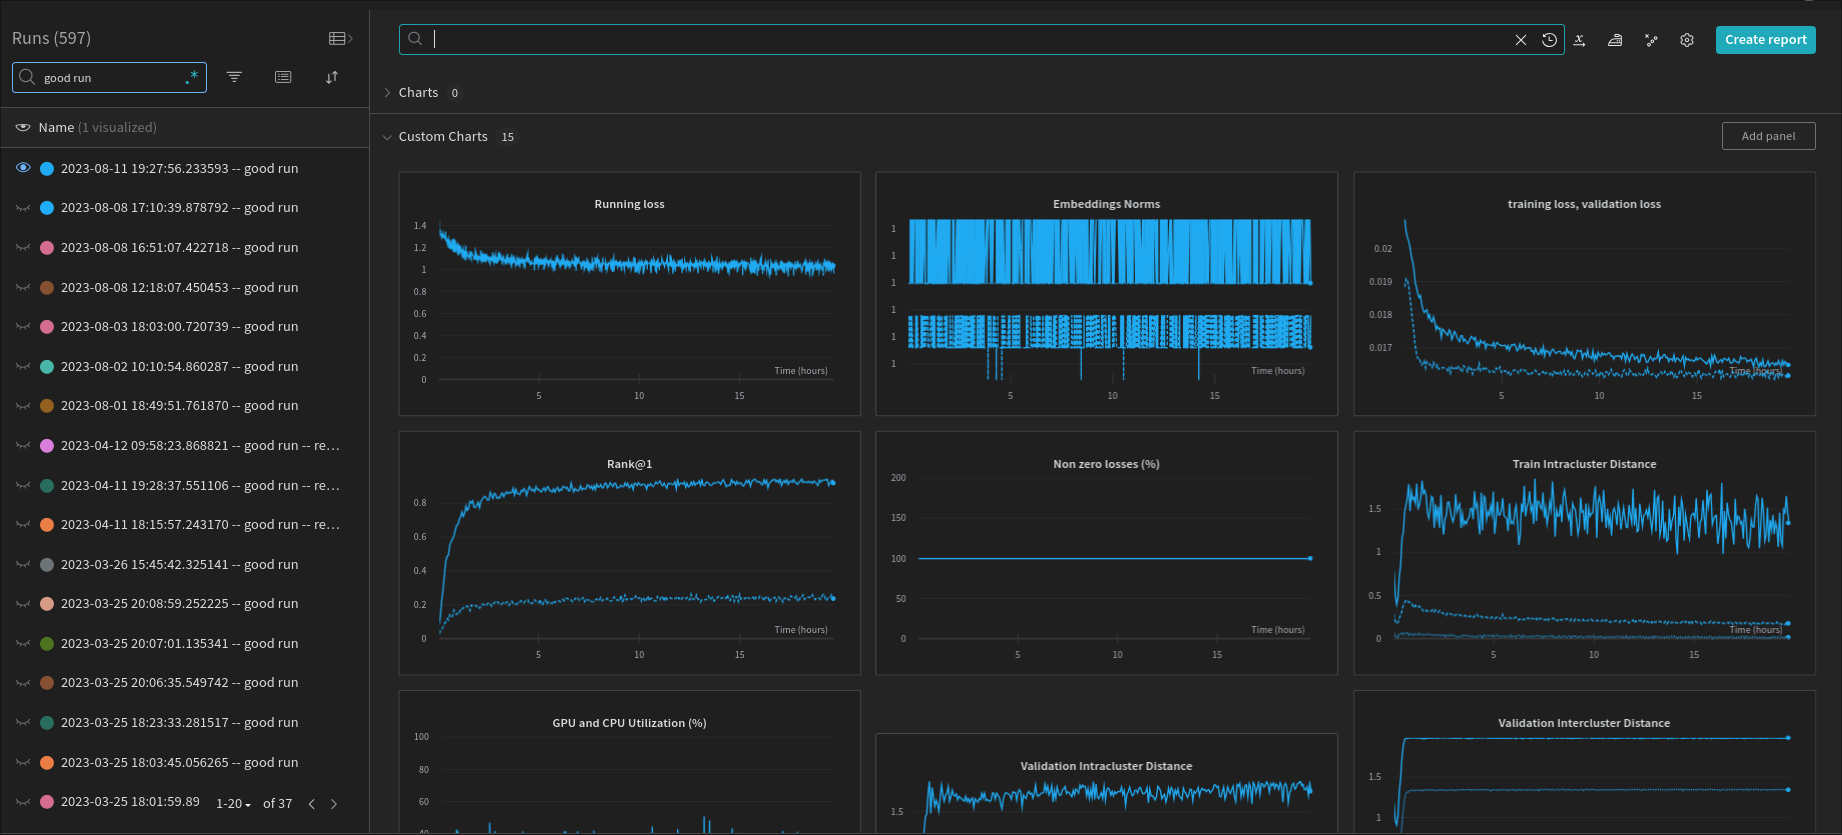
\includegraphics[width=0.8\textwidth]{informatica/wandb_example}
    \caption{Ejemplo de uso de \textit{WANDB}. A la izquierda, podemos ver una lista filtrada para mostrar solo los históricos que producen resultados satisfactorios. A la derecha, podemos ver algunas métricas recogidas por nuestro sistema de \textit{logging}}
\end{figure}

\section{Optimización del código} \label{isec:optimizacion_codigo}

Como ya se ha comentado en \customref{isec:planificacion}, una parte esperada del proceso de desarrollo es encontrar problemas de rendimiento, localizar qué partes del código están produciendo los problemas, y re-escribir implementaciones mucho más eficientes.

Además, en \customref{isubs:localizacion_partes_criticas} hemos justificado por qué es necesario realizar un \textit{profile} para identificar las secciones críticas del código. De otra forma, estaríamos realizando optimizaciones con muy poco impacto.

En esta sección explicamos cómo hemos desarrollado todo este proceso.

\subsection{Identificación del problema}

Identificamos problemas con los tiempos de cómputo por primera vez trabajando con el \textit{dataset} \textit{LFW}. El proceso de identificación y resolución se agrupan en las issues \cite{informatica:issue35_profiling} y \cite{informatica:issue36_slowmetrics}. Todo el proceso de optimización se resuelve en la \textit{pull request} \cite{informatica:pr42_profiling}. El \textit{commit} \lstinline{6aade342e07} \cite{informatica:commit_base_optimizacion} indica el estado original previo a realizar el proceso de optimización (\textit{profiling}, identificación de cuellos de botella, \textit{benchmarking} y cambios en las implementaciones).

\subsection{Organización del proceso}

El proceso de optimización se compone de los siguientes pasos:

\begin{itemize}
    \item \textit{Profiling} del código. Usamos la librería \lstinline{cProfile}. Esta forma parte de la librería estándar de \lstinline{Python}
    \item Identificación de los cuellos de botella. Para ello usaremos \lstinline{pstats} (que también forma parte de la librería estándar de \lstinline{python}) para explorar los resultados desde la terminal, y \lstinline{snakeviz} para explorar los datos de forma gráfica e interactiva
    \item Introducción de \textit{benchmarks} para medir los tiempos de ejecución en los cuellos de botella que vamos a modificar. Con ello tendremos mayor control sobre el impacto que suponen los cambios introducidos
    \item Realización de cambios sobre los cuellos de botella identificados y medición el impacto que suponen
\end{itemize}

En la sección de código donde realizamos el entrenamiento, añadimos la opción de usar la librería \lstinline{cProfile} para generar un \textit{profile}. Guardamos los resultados en la carpeta \lstinline{./src/profiling}, en los archivos \lstinline|{first, second, third}_profile.stat|.

Usando el paquete \lstinline{pstats} podemos realizar consultas sobre los archivos \lstinline{.stat}. Para ello usamos el comando \lstinline{python -m pstats <file_path>}. Tomamos el tiempo acumulado de cada función y guardamos los resultados en los archivos \lstinline|{first, second, third}_profile.txt|. Usando un editor de texto, filtramos esos archivos para que solo contengan entradas asociadas a funciones de nuestra librería (no nos interesan los tiempos de funciones de la librería estándar, por ejemplo) y guardamos el filtrado en los archivos \lstinline|{first, second, third}_profile_filtered.txt|. Con ello, podemos consultar estos resultados filtrados con un editor de texto, de forma más cómoda que trabajando con todos los resultados usando \lstinline{pstats}.

Usando el paquete \lstinline{snakeviz} podemos consultar de forma gráfica e interactiva los resultados almacenados en los archivos \lstinline{.stat}. Esto permite explorar los resultados de forma mucho más intuitiva, como veremos a continuación.

\subsection{Primer \textit{profile}}

En este \textit{profile} usamos los siguientes parámetros durante el ciclo de entrenamiento:

\begin{itemize}
    \item Enfoque \textit{lazy} para el aumentado de datos (véase \customref{isec:aumentado_datos})
    \item $P = 200$, $K = 2$
    \item Dimensión del \textit{embedding} a aprender igual a 5
\end{itemize}

Obtenemos los siguientes resultados, que visualizamos con \lstinline{snakeviz}:

\begin{figure}[H]
\centering
\ajustarsubcaptions

    \begin{subfigure}{.5\textwidth}
        \centering
        \includegraphics[width=0.9\linewidth]{informatica/profiles/first_profile/global}
        \caption{Visualización global de todo el proceso de entrenamiento}
        \label{img:first_profile_global}
    \end{subfigure}%
    \begin{subfigure}{.5\textwidth}
        \centering
        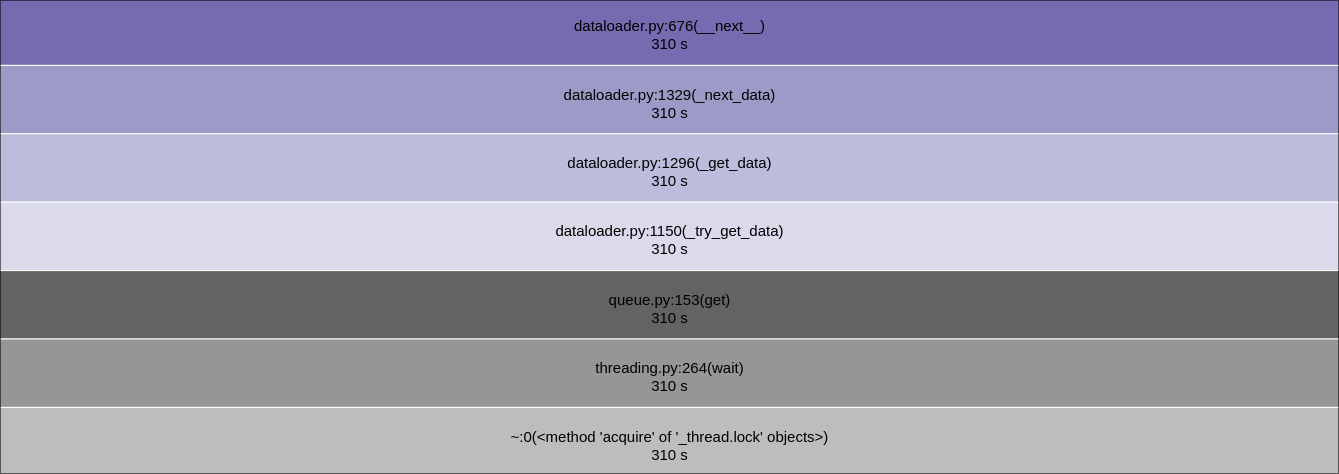
\includegraphics[width=0.9\linewidth]{informatica/profiles/first_profile/dataloader}
        \caption{Visualización de los tiempos involucrados en computar \lstinline{dataloader.__next__}}
        \label{img:first_profile_dataloader_next}
    \end{subfigure}
\caption{Visualizaciones obtenidas usando \lstinline{snakeviz} para los resultados del \textit{profile} inicial}
\end{figure}

El tiempo total de cómputo es de 328.638 segundos. Podemos ver en \customref{img:first_profile_global} que la mayor parte del tiempo de entrenamiento se dedica al método \lstinline{dataloader.__next__()}. En \customref{img:first_profile_dataloader_next} podemos ver que, en dicho método, prácticamente todo el tiempo estamos esperando a que se complete una operación asíncrona, como indica \lstinline{threading.wait()}.

Creemos que esto es por estar empleando el enfoque \textit{lazy} para el aumentado de datos. Cada vez que queremos acceder a una nueva imagen, tenemos que generarla en ese preciso instante. Por tanto, en la siguiente iteración no usaremos el enfoque \textit{lazy}. Veremos si los tiempos aumentan o disminuyen, y si aparecen nuevas partes de código a optimizar.

\subsection{Segundo \textit{profile}}

Como ya hemos comentado, esta vez nos centraremos en usar un enfoque no \textit{lazy} para el aumentado de datos. Si intentamos usar los mismos valores $P = 200$, $K = 2$, saturamos la memoria del proceso haciendo que este aborte. Así que tenemos que usar $P = 100, K = 2$, lo que supone un problema para comparar los nuevos resultados con los del primer \textit{profile}.

Para evitar que estas diferencias al cambiar los parámetros $\{P, K\}$ interfieran en nuestra optimización, lanzamos las dos versiones (\textit{lazy} y clásico) usando los valores $P = 100$, $K = 2$, y con ello podremos comparar de forma justa los tiempos de ejecución. Los resultados se resumen en la siguiente tabla:

\begin{table}[H]
\centering
\begin{tabular}{|l|l|l|}
    \hline
    \textbf{Enfoque} & \textbf{Tiempo total de ejecución (s)} & \textbf{Tiempo total de ejecución (min)} \\
    \hline

    \textit{Lazy} & 952.00s & 15.86 min \\
    Clásico       & 917.84s & 15.29 min \\

    \hline

\end{tabular}
\caption{Tiempos de ejecución de los dos enfoques de aumento de datos, usando los valores $P = 100, K = 2$}
\end{table}

Como era de esperar por lo comentado en \customref{isec:aumentado_datos}, el enfoque \textit{lazy} conlleva un tiempo de ejecución mayor. Solo estamos midiendo el tiempo de ejecución en el entrenamiento, no tenemos en cuenta los tiempos asociados a generar el \textit{dataset} aumentado. Y de esta forma, el enfoque clásico ya tiene todas las imágenes pre-computadas (lo que conlleva un tiempo considerable que no estamos teniendo en cuenta), mientras que el enfoque \textit{lazy} las tiene que generar a demanda. Sin embargo, acabamos de ver que el enfoque \textit{lazy} permite usar valores $\{P, K\}$ más altos. Y además, la diferencia no es demasiado grande: menos de un minuto de diferencia en tiempos totales de algo más de 15 minutos (sin considerar lo que tarda en generarse el \textit{dataset} aumentado de forma clásica).

Una vez resuelto esto, realizamos un segundo \textit{profile} usando los siguientes parámetros:

\begin{itemize}
    \item $P = 100$, $K = 2$
    \item Aumentado de datos clásico
    \item Dimensión del \textit{embedding} aprendido igual a 5
\end{itemize}

Los resultados del segundo \textit{profile} se muestran en la siguiente imagen:

\begin{figure}[H]
    \centering
    \includegraphics[width=0.8\textwidth]{informatica/profiles/second_profile/global}
    \caption{Visualización obtenida usando \lstinline{snakeviz} para los resultados del segundo \textit{profile}}
\end{figure}

En este caso, podemos ver que los resultados ya son más interesantes. Los tiempos de entrenamiento se dividen principalmente en dos bloques: el asociado a mostrar métricas con nuestra estructura de \textit{logging} (véase \customref{isec:loggin_metricas}) y el asociado al cálculo de la función de pérdida. Empecemos viendo el bloque de los \textit{loggers}:

\begin{figure}[H]
    \centering
    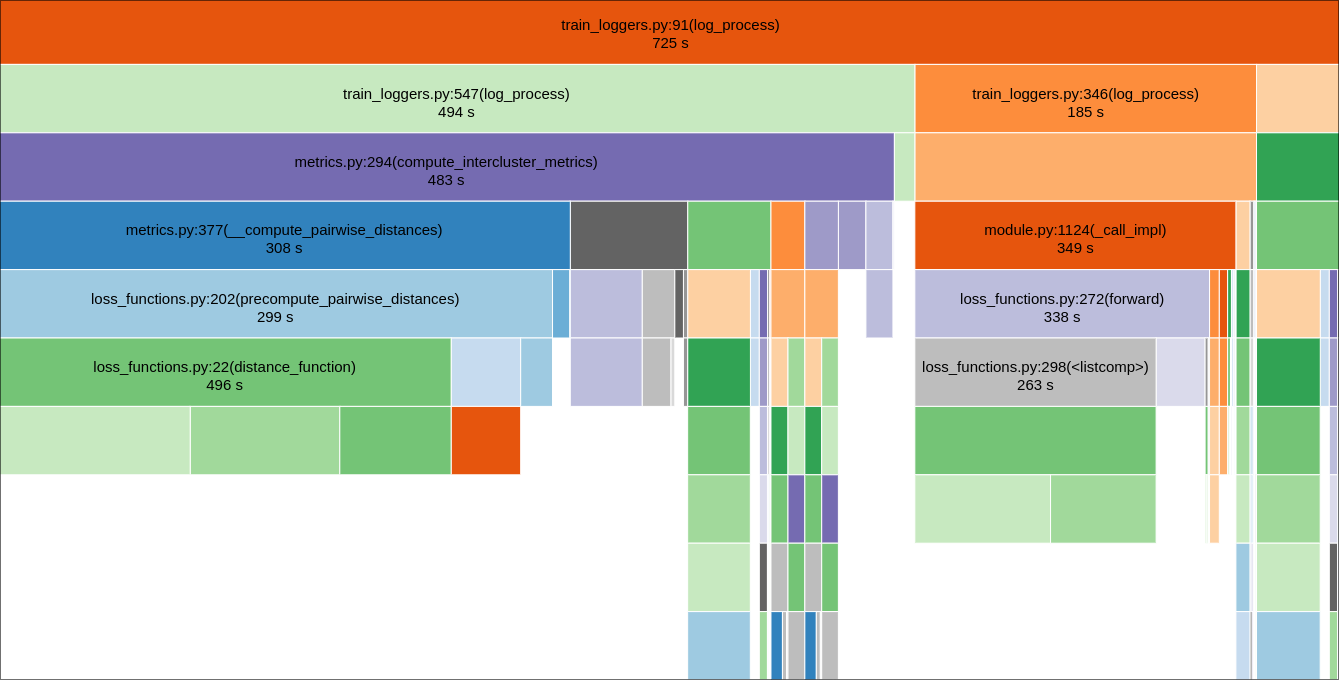
\includegraphics[width=0.8\textwidth]{informatica/profiles/second_profile/loggers}
    \caption{Visualización de los tiempos de cómputo asociados al \textit{logging} de métricas}
    \label{img:second_profile_tiempos_metricas}
\end{figure}

Podemos ver que la mayoría de tiempo se pasa en \lstinline{compute_intercluster_metrics} (métrica que introducimos en \customref{isubs:teoria_distancia_intra_inter_cluster}). Un gran porcentaje del tiempo de esta última función se gasta en pre-computar las distancias entre todos los pares de individuos. A su vez, gran parte del tiempo se gasta en computar la función de distancia \lstinline{distance_function} entre todos los pares de \textit{embeddings}.

Ahora estudiamos el bloque asociado al cálculo de la función de pérdida:

\begin{figure}[H]
    \centering
    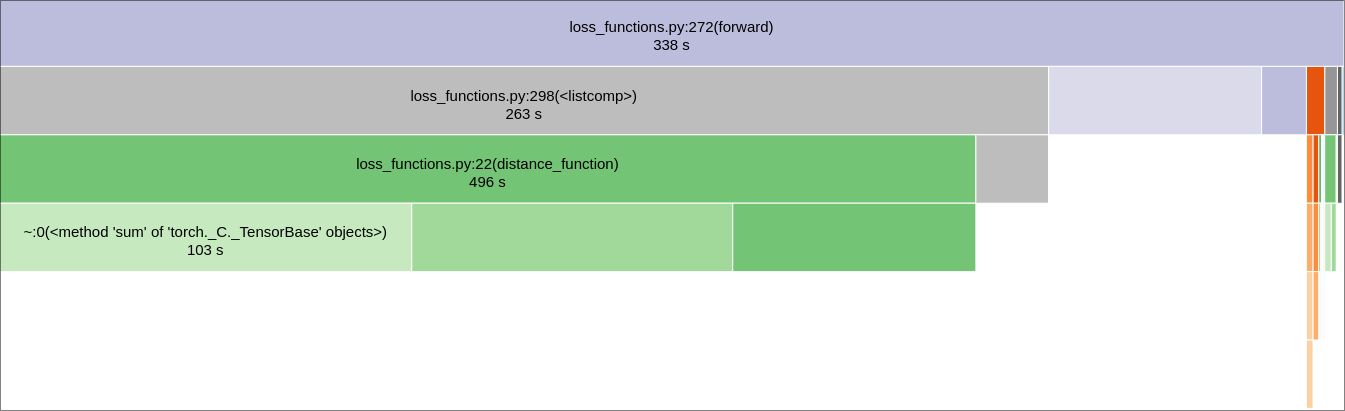
\includegraphics[width=0.8\textwidth]{informatica/profiles/second_profile/loss_function}
    \caption{Visualización de los tiempos de cómputo asociados al cálculo de la función de pérdida}
\end{figure}

Podemos ver que la mayor parte del tiempo se pasa en realizar una comprensión de lista (análogo a un bucle \lstinline{for}) para computar distancias entre todos los pares de puntos, como ya hemos visto en \customref{img:second_profile_tiempos_metricas}.

\subsection{Primera ronda de optimizaciones}

Con toda esta información, hemos localizado algunos cuellos de botella. Escribimos \textit{benchmarks} para estas partes del código previo a introducir cambios. Gracias a disponer de \textit{benchmarks}, estudiamos si estos cambios mejoran o empeoran los tiempos de cómputo.

Algunos detalles sobre los \textit{benchmarks}:

\begin{itemize}
    \item Estudiaremos los tiempos de ejecución de las funciones \lstinline{compute_intercluster_metrics} y \lstinline{precompute_pairwise_distances} con los dos \textit{scripts} que se encuentran en \lstinline{./src/benchmarks}
    \item Correremos estos \textit{scripts} en la plataforma \textit{Google Colab} (véase \customref{isec:entorno_ejecucion}), usando un \textit{Notebook} que invoca el código de los \textit{benchmarks}: \lstinline{./src/benchmarks/Benchmarking notebook.ipynb}
    \item Usaremos los parámetros:
        \begin{itemize}
            \item $P = 100, K = 2$
            \item Enfoque \textit{lazy} para el aumentado de datos
            \item Dimensión del \textit{embedding} a aprender igual a 5
            \item Una época de entrenamiento
        \end{itemize}
\end{itemize}

La siguiente tabla muestra los cambios introducidos y los tiempos de los \textit{benchmarks}. Además, mostramos el tiempo de ejecución del \textit{Notebook} \lstinline{LFW Notebook.ipynb}, que en el momento de realizar las optimizaciones, usábamos para entrenar y validar modelos sobre el \textit{dataset} \textit{LFW}.

\begin{table}[H]
    \centering
    \scalebox{0.8}{
    \begin{tabular}{lccccc}
        \toprule
        \textbf{} & \multicolumn{2}{c}{\textbf{\lstinline|compute_intercluster_metrics|}} & \multicolumn{2}{c}{\textbf{\lstinline|precompute_pairwise_distances|}} & \textbf{Tiempo entrenamiento} \\
        \cmidrule(lr){2-3} \cmidrule(lr){4-5}
        \textbf{Id. Cambio} & Media & Desv. Típica & Media & Desv. Típica & \\
        \midrule
        1 & 16.01 & 2.41 & 37.02 & 0.56 & 939.52 \\
        2 &  3.25 & 0.93  & 12.05 & 0.67 & 734.75  \\
        3 &  2.55 & 1.61  & 12.75 & 1.48 & 625.89  \\
        \bottomrule
    \end{tabular}
    }
    \caption{Tabla que recoge el proceso de optimización del código. Identificamos numéricamente los cambios realizados, que a continuación describiremos. Por cada cambio, vemos los nuevos resultados en los \textit{benchmarks}. También vemos el tiempo que tarda en completarse el ciclo de entrenamiento. Los tiempos de los \textit{benchmarks} se dan como un par (media, desviación típica). Damos los tiempos en segundos}
\end{table}

Los cambios realizados asociados a los identificadores numéricos son:

\begin{enumerate}
    \item Estado inicial de la base de código. No se han realizado cambios todavía. Los tiempos en este estado se toman como base a mejorar
    \item En \lstinline|precompute_pairwise_distances|, usamos el método \lstinline|cdist| de \lstinline|pytorch| para calcular una matriz de distancias. Convertimos dicha matriz a un diccionario para respetar la interfaz que ciertas clases esperan de esta función
    \item Usamos \lstinline|precompute_pairwise_distances| en el cálculo de las funciones de pérdida. Introducimos algunos pre-cómputos en \lstinline|compute_intracluster_distances| para acelerar la ejecución
\end{enumerate}

Podemos ver que los cambios introducidos mejoran los tiempos de cómputo de forma sustancial. Por tanto, estos cambios son relevantes y los mantenemos, aunque esto implique que algunas funciones sean más complicadas y menos legibles.

\subsection{Tercer \textit{profile}}

La primera ronda de optimizaciones potencialmente ha cambiado los cuellos de botella del código. Así que es necesario llevar a cabo un tercer \textit{profile} para estudiar el estado de la base de código e identificar, si hiciera falta, nuevos cuellos de botella a optimizar.

En este \textit{profile} usamos los siguientes parámetros:

\begin{itemize}
    \item $P = 100$, $K = 2$
    \item Una época de entrenamiento
    \item \textit{Embedding Dimension} = 1
    \item Enfoque \textit{Lazy} para el aumentado de datos
\end{itemize}

Visualizamos los resultados del \textit{profile} en la siguiente imagen:

\begin{figure}[H]
    \centering
    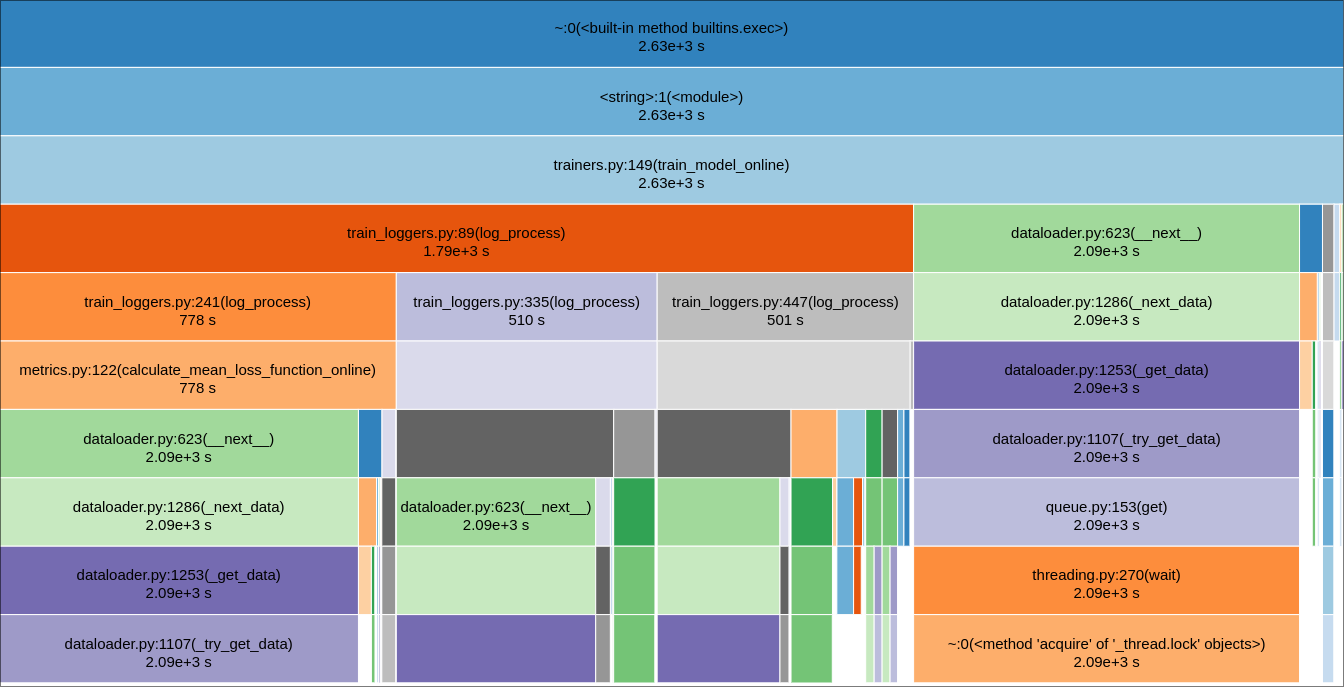
\includegraphics[width=0.8\textwidth]{informatica/profiles/third_profile/total}
    \caption{Visualización global de todo el proceso de entrenamiento.}
\end{figure}

Podemos ver que la mayor parte del tiempo se corresponde al \textit{logging} de métricas, seguido del acceso a los datos. Sobre el acceso de datos ya hemos trabajado, así que pasamos a estudiar en qué se gasta el tiempo en el \textit{logging}.


\begin{figure}[H]
    \centering
    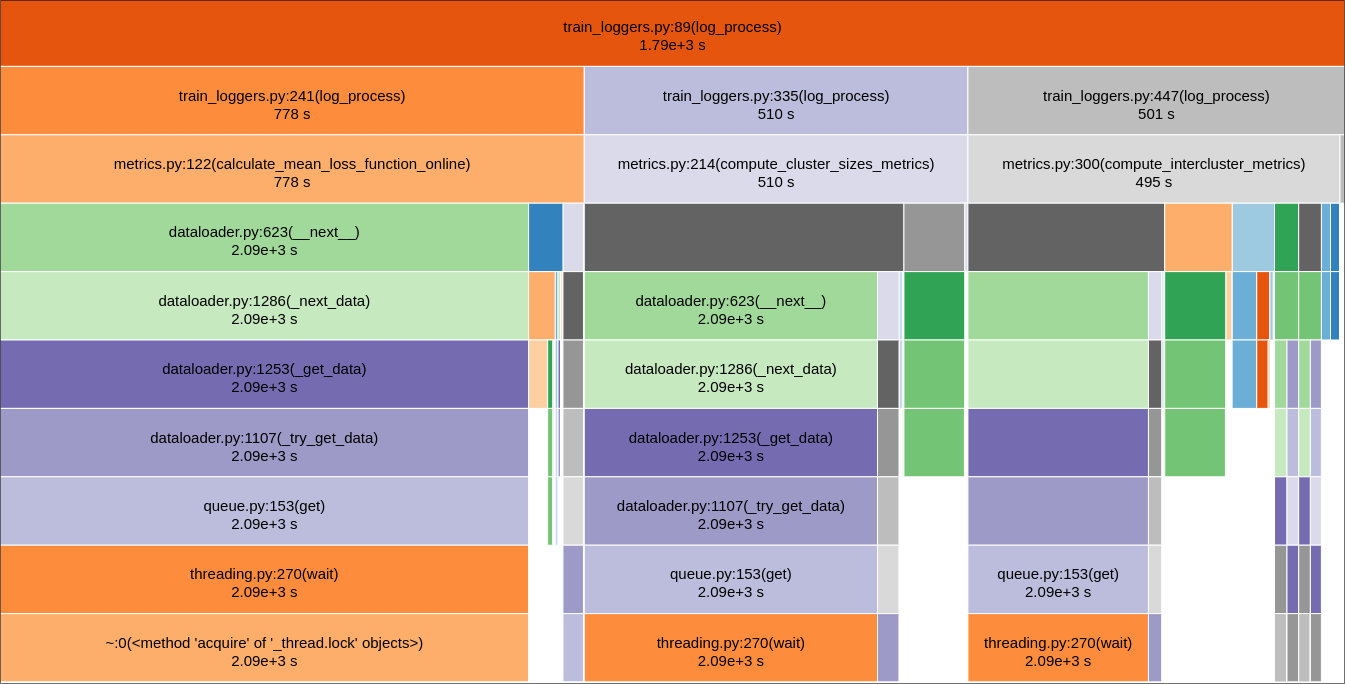
\includegraphics[width=0.8\textwidth]{informatica/profiles/third_profile/logging}
    \caption{Visualización de los tiempos de cómputo asociados al \textit{logging} de métricas}
\end{figure}

Tenemos tres bloques, que podemos expandir, como mostramos en las siguientes imágenes:

\begin{figure}[H]
\centering
    \begin{subfigure}{.5\textwidth}
        \centering
        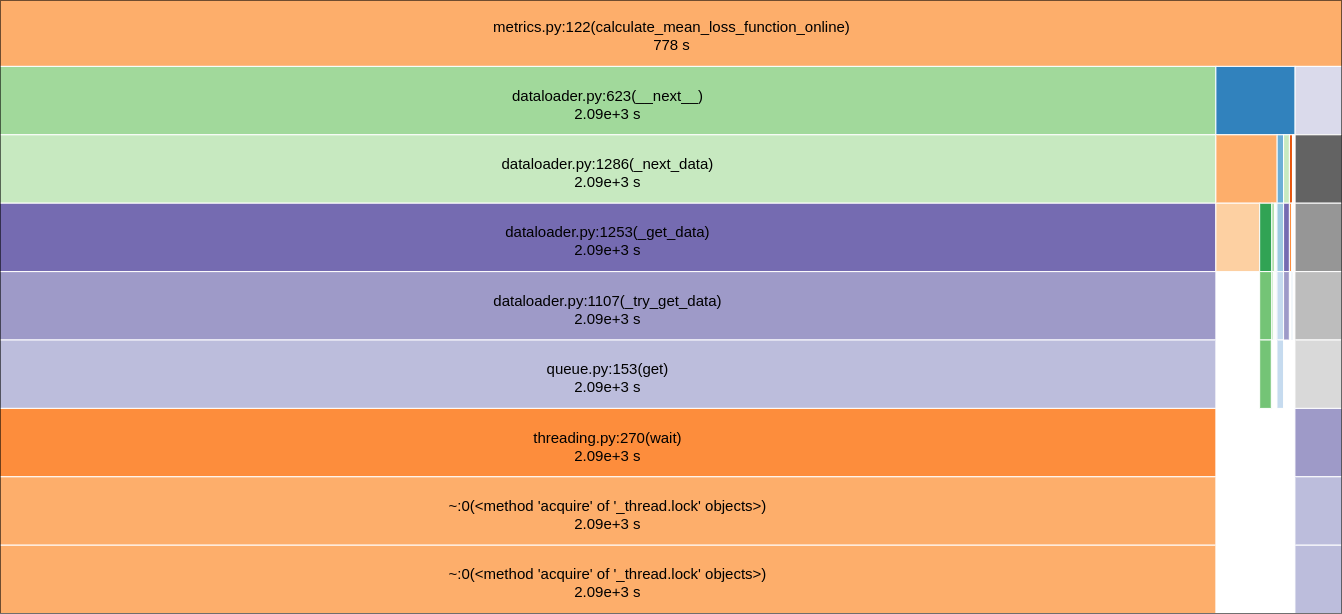
\includegraphics[width=0.98\linewidth]{informatica/profiles/third_profile/logging_primero}
        \caption{\lstinline{calculate_mean_loss_function_online}}
    \end{subfigure}%
    \begin{subfigure}{.5\textwidth}
        \centering
        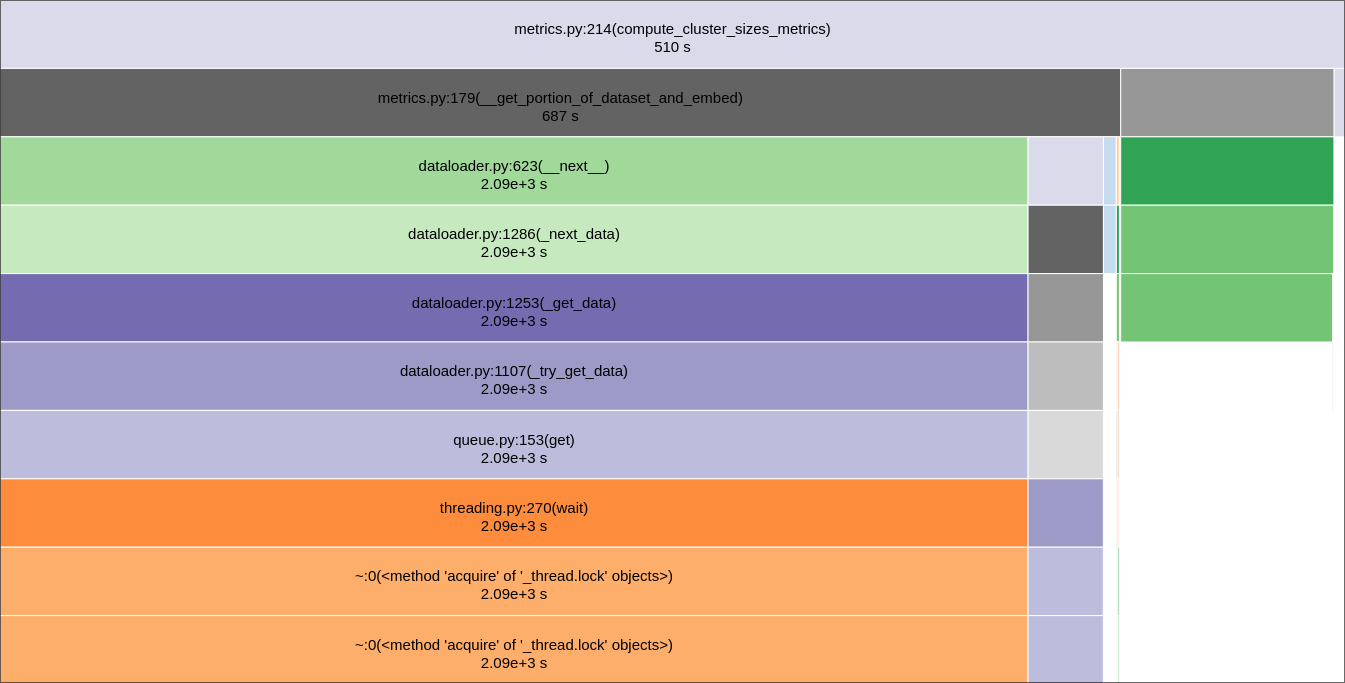
\includegraphics[width=0.98\linewidth]{informatica/profiles/third_profile/logging_segundo}
        \caption{\lstinline{compute_cluster_sizes_metrics}}
    \end{subfigure}

    \begin{subfigure}{.7\textwidth}
        \centering
        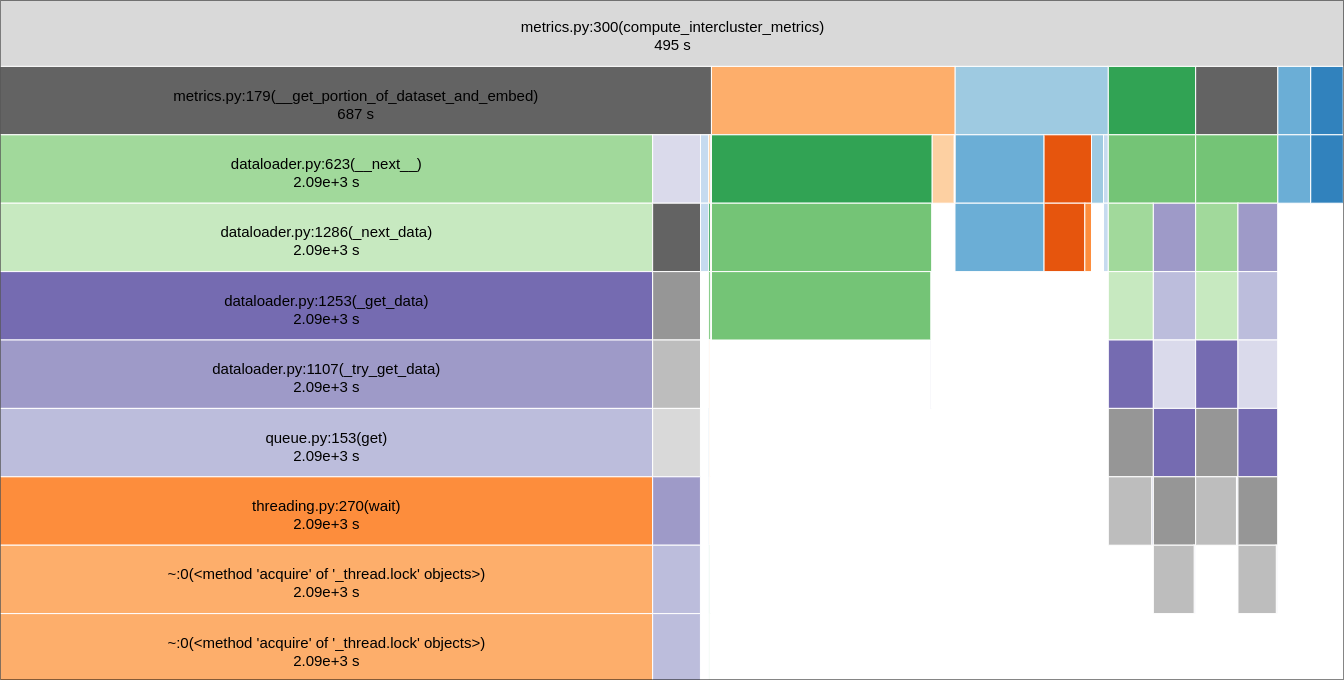
\includegraphics[width=0.8\linewidth]{informatica/profiles/third_profile/logging_tercero}
        \caption{\lstinline{compute_intercluster_metrics}}
    \end{subfigure}
\caption{Visualización de los tiempos de cómputo asociados a cada una de las tres métricas que mostramos}
\end{figure}

En base a estas visualizaciones podemos ver que:

\begin{sloppypar}
\begin{itemize}
    \item Las tres métricas que en ese momento estábamos mostrando suponen aproximadamente la misma cantidad de tiempo
    \item En \lstinline{calculate_mean_loss_function_online}, la mayor parte del tiempo se debe al acceso a los datos
    \item En \lstinline{compute_cluster_sizes_metrics}, la mayor parte del tiempo se pasa en \lstinline{__get_portion_of_dataset_and_embed}
    \item En \lstinline[breaklines=true]{compute_inter_cluster_metrics} la mayor parte del tiempo se pasa en \lstinline[breaklines=true]{__get_portion_of_dataset_and_embed}, pero no tanto como en el caso anterior. Le sigue la función \lstinline{__compute_pairwise_distances}
\end{itemize}
\end{sloppypar}

Además, estudiando el archivo con los tiempos de cómputo filtrados \lstinline{./src/profiling/third_profile_filtered.txt}, podemos ver que:

\begin{itemize}
    \item Como ya hemos visto, la mayor parte del tiempo se pasa en \lstinline{log_process}, seguido de \lstinline{calculate_mean_loss_function_online}, \lstinline{__get_portion_of_dataset_and_embed} y \lstinline{compute_cluster_sizes_metrics}
    \item Una comprensión de diccionarios en \lstinline{precompute_pairwise_distances} supone 1.524 segundos de 1.526 segundos que tarda la función en total
\end{itemize}

Todo esto justifica que identifiquemos las siguientes partes críticas del código, a tratar en una segunda ronda de optimizaciones:

\begin{itemize}
    \item \lstinline{calculate_mean_loss_function_online}
    \item \lstinline{__get_portion_of_dataset_and_embed}
        \begin{itemize}
            \item De esta forma, como ya hemos visto previamente, estaríamos optimizando tanto \lstinline{compute_cluster_sizes_metrics} y \lstinline{compute_intercluster_metrics}
        \end{itemize}
    \item Mejorar la comprensión de diccionarios en \lstinline{__compute_pairwise_distances}
\end{itemize}

\subsection{Segunda ronda de optimizaciones} \label{isubs:segunda_ronda_optimizaciones}

Seguimos el mismo enfoque que en la primera ronda de optimizaciones. Ya tenemos un \textit{benchmark} para \lstinline{compute_intercluster_metrics}. Como \lstinline{compute_intercluster_distances} se usa en \lstinline{compute_intercluster_metrics}, no añadimos un nuevo \textit{benchmark}, y veremos el impacto de los cambios a través del primer \textit{benchmark}.

\begin{table}[H]
    \centering
    \scalebox{0.8}{
    \begin{tabular}{lccccc}
        \toprule
        \textbf{} & \multicolumn{2}{c}{\textbf{\lstinline|compute_intercluster_metrics|}} & \multicolumn{2}{c}{\textbf{\lstinline|precompute_pairwise_distances|}} & \textbf{Tiempo entrenamiento} \\
        \cmidrule(lr){2-3} \cmidrule(lr){4-5}
        \textbf{Id. Cambio} & Media & Desv. Típica & Media & Desv. Típica & \\
        \midrule
            1 & 2.55  & 1.61 & 12.75 & 1.48 & 625.89  \\
            2 & 3.03  & 1.90 & 13.62 & 0.50 & -       \\
            3 & 3.45  & 2.68 & 13.28 & 0.37 & -       \\
        \bottomrule
    \end{tabular}
    }
    \caption{Tabla que recoge el segundo proceso de optimización del código. Identificamos numéricamente los cambios realizados, que a continuación describiremos. Por cada cambio, vemos los nuevos resultados en los \textit{benchmarks}. También vemos el tiempo que tarda en completarse el ciclo de entrenamiento. Los tiempos de los \textit{benchmarks} se dan como un par (media, desviación típica). Damos los tiempos en segundos}
    \label{table:optimization_process_second}
\end{table}

Describimos los cambios realizados:

\begin{enumerate}
    \item Estado inicial de la base de datos. No se han realizado cambios todavía. Los tiempos en este estado se toman como base a mejorar
    \item Refactorizamos \lstinline{__get_portion_of_dataset_and_embed} para usar una única llamada de \lstinline{pytorch} para computar todos los \textit{embeddings}, en vez de usar un bucle \lstinline{for}.
    \item Mejoramos el diseño de la anterior función. No deberían producirse cambios en el rendimiento
\end{enumerate}

En \customref{table:optimization_process_second} podemos ver que no estamos mostrando tiempos de cómputo de entrenamiento en las dos últimas entradas. Esto es porque el uso de la función de \lstinline{pytorch} para computar todos los \textit{embeddings} de golpe provoca que el consumo de memoria se eleve hasta abortar el proceso. Además, los \textit{benchmarks} han empeorado algo.

Sin embargo, mantenemos las dos implementaciones, permitiendo elegir cuál usar en cada momento. Puede ser que al acceder a los servidores \textit{nGPU} (véase \customref{isec:entorno_ejecucion}), mucho más potentes, la nueva implementación no provoque consumos elevados de memoria y acelere el proceso.

\subsection{Comentarios y mejoras a tener en cuenta}

En el momento de realizar este proceso de optimización, no teníamos acceso a los servidores \textit{nGPU}. Sin embargo, era necesario optimizar el código para seguir avanzando el proyecto sin detenernos.

El haber realizado la optimización sobre \textit{Google Colab} y no sobre los servidores \textit{nGPU} sobre los que finalmente correremos el aprendizaje y validación de modelos es un \textbf{error a tener en cuenta}. Por ejemplo, en \customref{isubs:segunda_ronda_optimizaciones} podemos ver que las conclusiones no son del todo robustas al trabajar en un entorno inferior y ser conocedores de que en futuro usaríamos un entorno mucho más potente. Por tanto, \textbf{una posible mejora} es repetir el proceso de optimización sobre los servidores \textit{nGPU}.

Sin embargo, al acceder a los servidores \textit{nGPU} y \textit{datasets} más grandes, no hemos tenido problemas de rendimiento. Con ello, un esfuerzo en optimizar el código no estaría del todo justificado. Por tanto, aún con los fallos que hemos comentado, \textbf{el proceso de optimización cumplió con su cometido} en el momento en el que era necesario.

\section{Pipeline} \label{isec:pipeline}

En Aprendizaje Automático, nos referimos por \textit{pipeline} a la descripción e implementación de las distintas fases o etapas que participan en la creación de un modelo \cite{informatica:pipeline_web}.

Existen múltiples soluciones para codificar estos \textit{pipelines}. Estas soluciones se encargan de facilitar la definición de los \textit{pipelines} y la automatización de ciertas tareas. Con estas soluciones podemos, por ejemplo, lanzar todo el proceso cada vez que se actualiza la base de datos, rechazar el nuevo modelo producido si este no cumple con ciertos criterios de calidad, desplegar en producción nuevos modelos, ...

Sin embargo, por la simplicidad de nuestro \textit{pipeline}, codificamos manualmente este proceso. Simplemente, usaremos variables globales, almacenadas en la variable \lstinline{GLOBALS} (véase \customref{isec:loggin_metricas}), para decidir si ejecutar o no ciertas secciones opcionales.

El siguiente diagrama describe el \textit{pipeline} seguido en todos nuestros experimentos:

\begin{figure}[H]
\centering
\scalebox{0.9}{
\begin{tikzpicture}[
    mandatorynode/.style={rectangle, draw=cyan!60, fill=cyan!5, very thick, minimum size=5mm, align=center},
    optionalnode/.style={rectangle, draw=green!60, fill=green!5, very thick, minimum size=5mm, align=center},
]
    \node [mandatorynode] (wandb) {\textit{Log} en \textit{WANDB}};
    \node [mandatorynode] (dataset_download) [right=of wandb] {Descarga de los datos};
    \node [mandatorynode] (dataset_load) [right=of dataset_download] {Carga de los datos en \\ un \lstinline{Dataset} de \lstinline{pytorch}};
    \node [mandatorynode] (dataset_split) [below=of dataset_load] {Dividir en \textit{train, test, validation}};
    \node [mandatorynode] (dataloaders) [left=of dataset_split] {Cargar los tres conjuntos de \\ datos en \lstinline{Dataloaders} de \lstinline{pytorch}};
    \node [optionalnode] (data_augmentation) [left=of dataloaders]{\textit{Data Augmentation}};
    \node [optionalnode] (hp_tuning) [below=of data_augmentation] {\textit{Hyperparameter Tuning}};
    \node [optionalnode] (train) [right=of hp_tuning] {Entrenamiento del modelo};
    \node [mandatorynode] (eval) [right=of train] {Evaluación del modelo};

    \draw[-stealth] (wandb.east) -- (dataset_download.west);
    \draw[-stealth] (dataset_download.east) -- (dataset_load.west);
    \draw[-stealth] (dataset_load.south) -- (dataset_split.north);
    \draw[-stealth] (dataset_split.west) -- (dataloaders.east);
    \draw[-stealth] (dataloaders.west) -- (data_augmentation.east);
    \draw[-stealth] (data_augmentation.south) -- (hp_tuning.north);
    \draw[-stealth] (hp_tuning.east) -- (train.west);
    \draw[-stealth] (train.east) -- (eval.west);

\end{tikzpicture}
}
\caption{Representación gráfica de nuestro \textit{pipeline}. Los nodos azules son nodos obligatorios. Los nodos verdes son nodos opcionales: usando \lstinline{GLOBALS} podemos decidir si ejecutarlos o no}
\end{figure}

Es claro que podemos saltarnos el proceso de aumento de datos y el \textit{hyperparamenter tuning}. De hecho, este último lo ejecutaremos muy pocas ocasiones. Sin embargo puede extrañar que hayamos marcado el entrenamiento del modelo como un paso opcional.

Cuando terminamos el entrenamiento de un modelo, guardamos los parámetros de dicho modelo en disco. Podemos recuperar ese modelo sin tener que pasar por todo el proceso de entrenamiento, y evaluarlo. Esto es útil por varias razones:

\begin{itemize}
    \item Si estamos desarrollando nuevas métricas, y queremos ver cómo funcionan en modelos entrenados, no tenemos que re-entrenar un modelo cada vez que introducimos un cambio en la métrica con la que estamos trabajando
    \item Podemos verificar que un modelo entrenado en el pasado obtiene ciertos valores de las métricas
    \item Al introducir una nueva métrica, podemos computarla para modelos entrenados previamente a la implementación de dicha métrica
\end{itemize}

\section{\textit{Suite} de \textit{tests}} \label{isec:test_suite}

Disponemos de dos conjuntos o \textit{suites} de \textit{tests}: \textit{tests} unitarios y \textit{tests} de integración.

Los \textbf{\textit{tests} unitarios} buscan principalmente validar la corrección de los módulos de código desarrollados en la librería. Para ello, usamos algunas técnicas comunes de \textit{testeo}:

\begin{itemize}
    \item Validación de casos concretos: controlamos los datos de entrada de una funcionalidad, y comprobamos la salida con el resultado esperado. Esto es factible cuando las funciones a validar son deterministas y fáciles de calcular manualmente. Como puede ser el caso de las funciones de pérdida, validadas en \lstinline{src/test/loss_functions.py} usando principalmente este enfoque
    \item Validación de propiedades \cite{informatica:property_based_testing}: dados unos datos de entrada, comprobamos que ciertas propiedades de la funcionalidad a validar se cumplen. Esta técnica es realmente útil cuando usamos funciones no deterministas, o cuando no es viable computar manualmente la salida esperada. Como puede ser el caso del aumentado de datos (véase \customref{isec:aumentado_datos}), de naturaleza claramente aleatoria. Comprobamos propiedades como:

    \begin{itemize}
        \item Que el tamaño del \textit{dataset} no aumenta si todos los individuos tienen al menos $K$ imágenes asociadas
        \item Que tras el aumento de datos todos los individuos tienen al menos $K$ imágenes asociadas
        \item Que el tamaño del \textit{dataset} aumenta o se mantiene, nunca disminuye
    \end{itemize}

\end{itemize}

También usamos \textit{tests} unitarios cada vez que encontramos un error en nuestra base de código, siguiendo el siguiente proceso:

\begin{itemize}
    \item Aislamos el error en una serie de \textit{tests} que comprueban la propiedad que no se está cumpliendo
    \item Tratamos de localizar y arreglar la fuente del error
    \item Comprobamos que, tras arreglar el problema, los \textit{tests} introducidos ahora sí que se ejecutan correctamente
\end{itemize}

Esto permite encontrar y solucionar los problemas más rápidamente, y además documentar errores previamente encontrados y propiedades que son importantes verificar en otros escenarios.

Los \textbf{\textit{tests} de integración} buscan evitar el siguiente problema. Como hemos comentado en \customref{isec:planificacion}, hemos realizado un trabajo iterativo, partiendo de conjuntos de datos más sencillos hacia conjuntos de datos más grandes y complejos. En dicho trabajo iterativo puede ocurrir que, cambiando o añadiendo código a la librería, rompamos \textit{pipelines} en conjuntos de datos previos. Los \textit{tests} de integración buscan verificar que \textit{pipelines} en conjuntos de datos previos sigan funcionando.

Para esto, cada \textit{test} de integración ejecuta el \textit{pipeline} de un conjunto de datos cuando abandonamos este para pasar al siguiente. Usamos valores de los parámetros para adecuar la tarea: usamos un subconjunto muy reducido de la base de datos, hacemos \textit{logging} de forma mucho menos frecuente, los valores de $\{P, K\}$ son más bajos, la red neuronal es muy ligera, ...

Por el esfuerzo computacional que suponen, los \textit{tests} de integración únicamente se ejecutan a la hora de validar una \textit{pull request}.

Y como ya hemos comentado en \customref{isec:github_buenas_practicas}, estamos usando \textit{Github Actions} para lanzar las dos \textit{suites} de \textit{tests}, aunque usando la herramienta \lstinline{just} (véase \customref{isec:estructura_carpetas}) se pueden lanzar en local.
